%% 
\chapter{Optimizing Species-Specified Aerosol Emissions from Satellite
Measured Radiances} \label{chap:optems}

\section{Introduction}

Tropospheric aerosols play an important role in the Earth’s energy budget and
hydrological cycle by directly scattering or absorbing solar radiation
(direct effect) and indirectly altering the cloud microphysical
properties and lifetime through serving as cloud condensation nuclei
(indirect effect) \citep{Haywood00}. The Intergovernmental Panel on
Climate Change \citep{IPCC07} reported direct and indirect aerosol
radiative forcing as --0.5 and --0.7 Wm$^{-2}$, respectively, both with 
uncertainty of about 100\%. Such large uncertainties are attributed not only 
to a diversity of representations of aerosol microphysical and optical 
properties across models \citep{Schulz06}, but also to the uncertainty in the 
emissions of aerosol particles and aerosol precursors (hereafter aerosol 
emissions) from both natural and anthropogenic sources.  Differences in global
aerosol emission estimates, ranging from 22\% to over 200\% depending on the 
species, were found among various global chemistry transport models (CTMs) 
\citep{Textor06}, highlighting the need to further improve the quantifications
of aerosol emissions. At regional scales, the emission inventories have much
larger uncertainty \citep{Streets03} and often don’t resolve the seasonal or
monthly variations, making it difficult to model regional climate, air quality
and visibility. In addition, accurate and timely knowledge of aerosol sources
is required for use of air quality models for studying impacts of aerosols on
human health \citep{Pope09}.

 Current estimates of aerosol emissions are largely based on the “bottom-up” 
method that integrates diverse information such as fuel consumption in various
industries and corresponding measurements of emission rates for different
species \citep{Streets03}, economic growth, and the statistics of land use
and fire-burned areas \citep{vanderWerf06}. While significant progress has
been made \citep{Streets06}, the “bottom-up” approach has a number of 
limitations. First, the emission inventory usually has a temporal lag of at
least 2 to 3 years, as time is needed to aggregate information from different
sources and format them into the emission inventories that are suitable for 
use in climate models. Second, the temporal resolution of the current emission
inventory is usually on monthly to annual scale, which is not sufficient to 
characterize the daily or diurnal variation of emissions; the aerosol impact 
on radiative transfer and the variation of cloud properties,  however, is 
often strongly dependent on the time of the day \citep{Wang06}. Third, the
spatial resolutions of the bottom-up emission inventories are usually 
limited by the availability of the ground-based observations, which often lack
the spatial coverage for estimating emission in a uniformly fine resolution 
for regional modeling of aerosol transport. Finally, bottom-up emission 
inventories may miss important emission sources that are not well documented 
including emissions from wild fires, volcanic eruptions, and agricultural 
activities. All these limitations are amplified over the East Asia region
 because the economic growth in China is so rapid that information needed
 for bottom-up approach cannot be timely and reliably documented.

 To complement information from bottom-up emissions, remote sensing is 
increasingly used to better quantify aerosol distributions. The satellite 
observations and/or products can provide information important for the 
bottom-up estimate of emissions. Examples include the fire products from 
MODIS, ASTER, and AVHRR sensors that are widely used for characterizing the 
biomass burning emissions \citep{Borrego08, vanderWerf06, vanderWerf10,
Reid09}. Alternatively, the satellite observed tracer abundance could be used
to constrain bottom-up estimates of aerosol emissions through the inverse 
modeling; such method is referred to as a ‘top-down’ constraint.
Although satellite-based aerosol retrievals have less precision than in situ 
measurements, studies have shown that they are able to quantify the 
atmospheric aerosol loading and temporal variations with good agreement and 
expected accuracy to the ground-based observations \citep{Levy10,
Remer05}. Furthermore, the satellite-based aerosol data, in contrast to the 
ground-based ones, have much higher temporal resolution across the globe. 
For instance, the MODIS sensor, aboard on NASA’s both Terra and Aqua 
satellites, has a surface footprint size of about 1 km at nadir and needs 
only 1 to 2 days to achieve global coverage. In addition, the joint retrieval
of aerosols from diverse satellite sensors enhances the accuracy of satellite
aerosol products \citep{Sinyuk08}, the potential of which have also been
shown in the air quality monitoring \citep{Liu05, Wang10}.

 Different top-down techniques have been developed to optimally estimates
the emissions from satellite observations, which include but are not limited 
to the following:
(a) the use of a scaling factor that is the ratio of observed tracer 
abundances to the CTM simulated counterparts \cite{Lee11, Martin03a, Wang06};
(b) the use of the local sensitivity of change of tracer concentration to the
change of emission \citep{Lamsal11, Walker10}; 
(c) the analytical Bayesian inversion method \citep[e.g.,][]{Heald04};  
(d) the adjoint of CTM \citep[e.g.,][]{Muller05, Henze07, Henze09,
Dubovik08, Kopacz09, Kopacz10, Wang12}.
The first two methods are similar; both assume a linear relationship between
model simulated aerosol abundances and emissions. The analytical method is
exact but computationally expensive and thus can only constrain emission in 
the domain-wise or over coarse spatial resolution \citep{Kopacz09}.
In contrast to the first three approaches, the adjoint approach is designed
for exploiting the high-density of observations to constrain emission
with high resolution, as it is able to efficiently calculate gradients of 
the overall mismatch between observations and model estimates with respect to
large sets of parameters (i.e., emissions resolved at each grid box) 
\citep{Henze07}.

 Several studies have successfully analyzed sources of traces gases using the
top-down methods, including \ce{CO} sources from MOPITT sensor over the Asia
\citep{Heald04, Kopacz09} and over the globe \citep[e.g.,][]{Stavrakou06, 
Kopacz10}, \ce{CO2} surface flux from the TES sensor \citep{Nassar11}, 
\ce{NOx} emissions from space-based column \ce{NO2} by several satellite 
sensors \citep{Lamsal11, Lin10, Martin03a, Muller05}, and \ce{SO2} from 
SCIAMACHY and OMI sensors \citep{Lee11}, etc. However, not all emissions of
trace gases can be fully constrained with their satellite-based counterpart 
products, because some trace gases (e.g. \ce{SO2}) can react with other gases
(e.g., \ce{NH3}), to form either liquid or solid aerosols 
(e.g., \ce{(NH4)2SO4}). As a result, using measurements of trace gases alone 
can only provide partial constraints on the emission of the corresponding 
trace gases.

Ultimately, combined use of measurements of both trace gases and aerosols 
should provide stronger constraint (than each individual measurement alone) for
the emission of aerosols and their precursors including trace gases. Unlike a
given trace gas, aerosol has complex chemical composition. Aerosol optical
depth (AOD), the only parameter that current satellite remote sensing can
provide and is well validated, contains little information on aerosol
composition. Consequently, assumption of aerosol composition is often made when
using AOD to constrain aerosol models. Examples from previous studies have
focused on assimilation of AOD to constrain model AOD \citep{Wang04,
Zhang08, Benedetti09}, or to estimate PM$_{2.5}$ concentrations
\citep{vanDonkelaar08}. While valuable for forecasts or estimating
distribution of aerosols, these studies do not provide direct constraints on
aerosol sources. In terms of constraining sources, a recent study by
\citep{Dubovik08} constrained aerosol primary sources in single-fine and 
single-coarse modes respectively from MODIS retrieved fine and coarse mode 
0.55 $\mu$m AOD by inverting the GOCART aerosol transport model. To overcome 
the inconsistency of aerosol single scattering properties between CTM and 
aerosol retrieval algorithm that may compromise the use of satellite AOD to 
quantitatively invert aerosol emissions, \citet{Weaver07} suggested directly
assimilating the satellite observed radiance (such as from MODIS) to improve
the CTM (GOCART model) simulation of aerosols. Improved retrieval of AOD and
improved estimate of surface PM concentration were also obtained by
\citet{Drury08} over the U.S. and \citet{Wang10} over China, when the 
GEOS-Chem simulated aerosol single scattering properties is used in the 
retrieval, allowing MODIS radiance to directly constrain the GEOS-Chem 
columnar mass of aerosols. Built upon this progress, we \citep{Wang12} 
further used MODIS radiance to constrain dust emissions over the East Asia.

 In this study, we present a new attempt for the top-down estimate 
 of aerosol emissions through integration of the satellite observation 
 of reflectance and GEOS-Chem Adjoint model. 
 The technique is applied to improve estimates of mineral dust 
 and anthropogenic \ce{SO2}, \ce{NH3}, \ce{NOx}, \ce{BC} and \ce{OC} 
 emissions over China for April 2008, during which ground-based 
 PM\textsubscript{10} (particulate matter with aerodynamic diameter of 
 10 $\mu$m or less) data is available from a joint China-U.S. 
 dust field experiment \citep{Huang10}. 
 This study differs from the past work in that: 
 (i) satellite reflectance (in essence radiance) is used 
 to constrain the emission estimates of aerosol particle and precursors, 
 which eliminates the discrepancy of aerosol optical properties 
 between model simulated and satellite retrieved AOD; 
 (ii) we use a suite of aerosol and gas measurements 
 from satellite sensors and ground-based instruments 
 to independently evaluate our results, and test our hypothesis 
 that temporal variation of AOD at different locations, 
 as characterized by satellite observations, can be a strong constraint 
 for species-specific source estimates if they are combined with 
 the model-based knowledge of the dominant aerosol sources 
 and the source-receptor relationship at corresponding locations; 
 and (iii) combination of (i) and (ii) will provide the basis and 
 a necessary step forward for future research to simultaneously 
 use both gas and AOD measurements to constrain speciated aerosol emissions. 

 We present the general structure of our inversion methodology in
section \ref{sec:generalstr}, in which we describe the observation 
constraints and the inversion strategies. The top-down constraints on aerosol 
emissions over China for the period of April 2008 are presented in 
section \ref{sec:invresult},  and evaluated by indepdent observation acquired 
from various platforms in section \ref{sec:invevaluation}. Interpretation and
implications of the results are discussed in section \ref{sec:invimplication},
and section \ref{sec:invsummary} summaries this work.

\section{Observational Constraints and Inversion Methodology} 
\label{sec:generalstr}

 As shown in Figure \ref{fig:flowchat}, the top-down inversion approach in 
this study integrates the MODIS radiance/reflectance with the GEOS-Chem 
(section \ref{subsec:gc}) and its adjoint model (section \ref{subsec:gcadj}) 
to optimize aerosol emissions. First, similar to \citet{Wang10}, we retrieve
the atmospheric aerosol mass and AOD through fitting the calculated radiance
based on GEOS-Chem aerosol composition and single optical properties to the 
MODIS cloud-free radiances (section \ref{subsec:modisobs}). Second, the 
retrieved AOD (hereafter retrieved MODIS AOD) from the first step is used as 
an observational constraint to optimize the aerosol emissions by inverting the
GEOS-Chem chemical transport model. The approach aims to improve aerosol 
emission estimates that ultimately will yield better agreement between model
simulated and satellite-observed reflectances.  Since the aerosol single 
scattering properties are exactly the same between the retrieval algorithm and
GEOS-Chem (as done in the first step), the top-down inversion scheme 
essentially uses the MODIS radiances (in the form of retrieved AOD) to scale 
the GEOS-Chem aerosol mass, which in turn are used to optimally adjust  the 
aerosol emissions. The approach here is first demonstrated through a 
pseudo-observation experiment (section \ref{subsec:pseudo}) before it is 
applied to real observations (Section \ref{sec:invresult}).

 \begin{figure}[t]
  \centering
  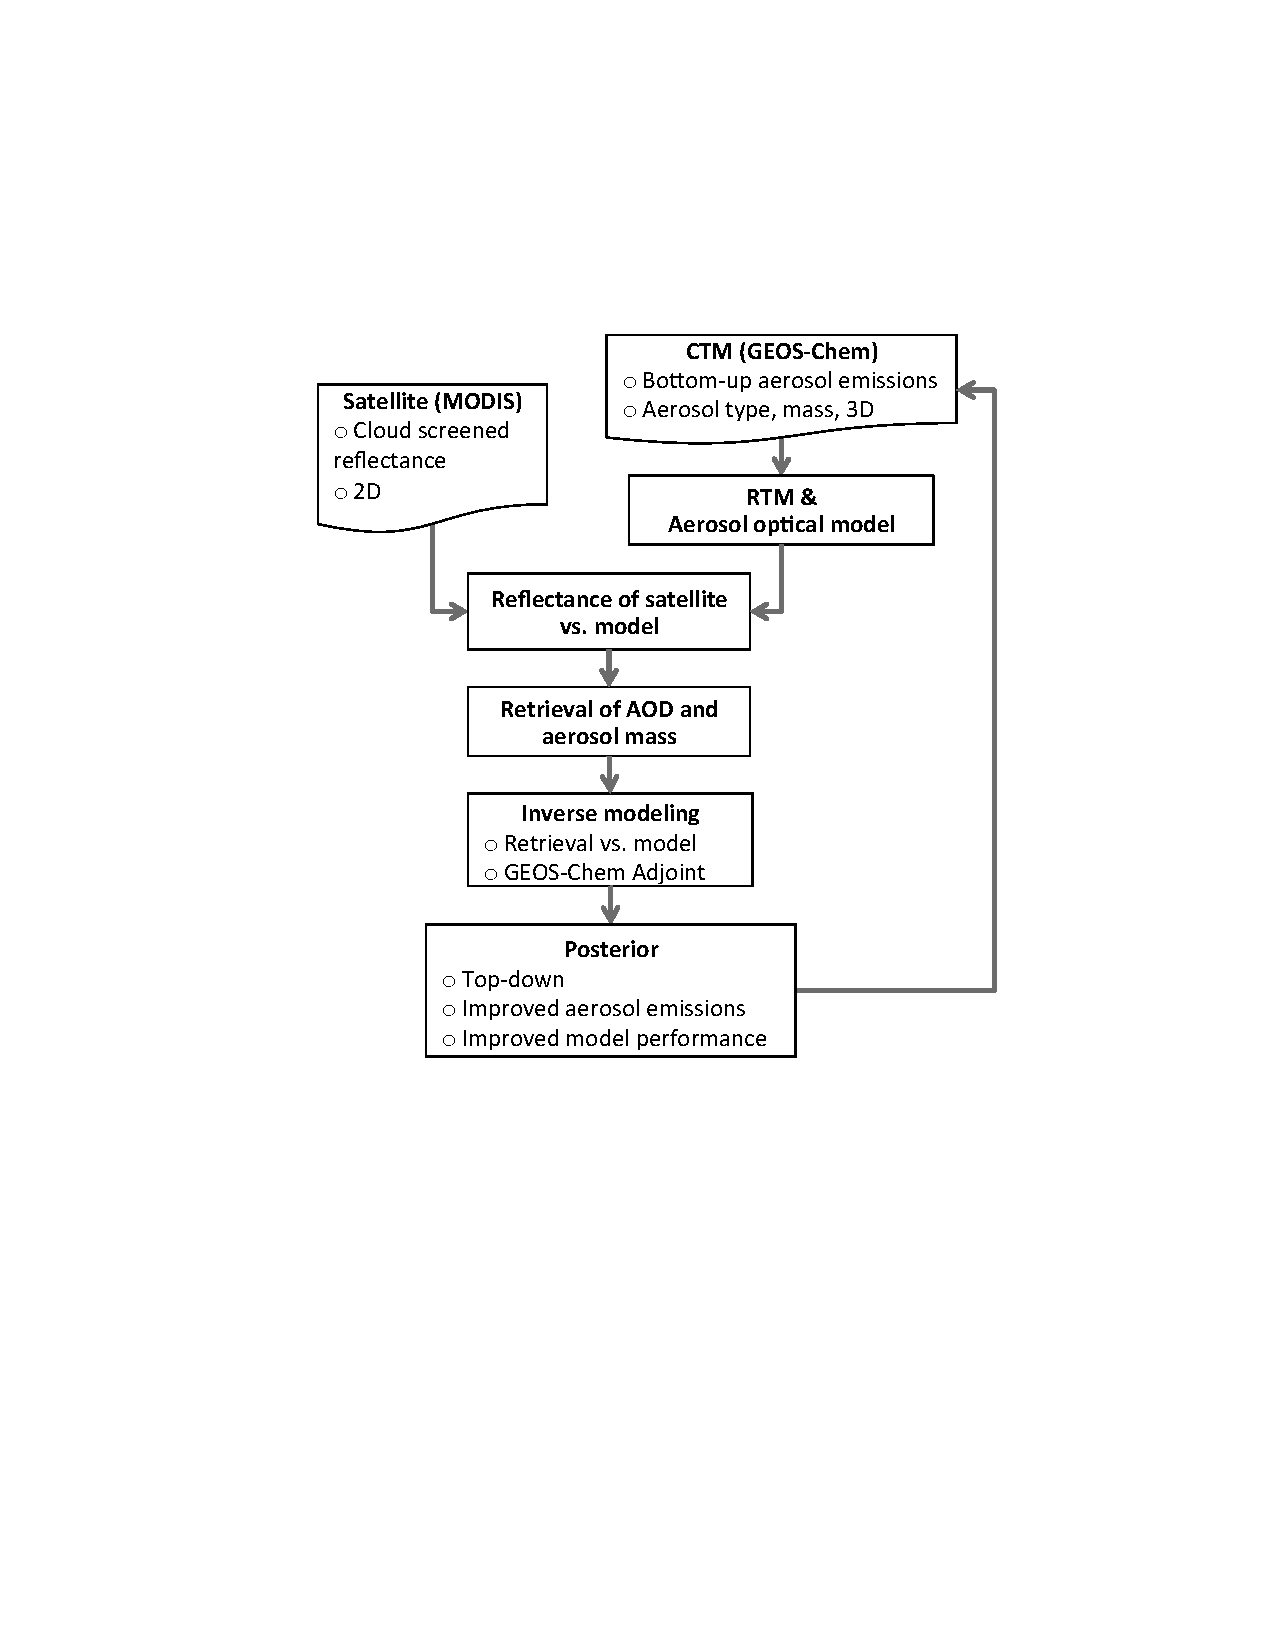
\includegraphics[width={0.7\textwidth}]{figures/a1.pdf}
  \caption{Flowchart of the proposed top-down inversion framework \citep{Xu13}.}
  \label{fig:flowchat}
 \end{figure}

\subsection{GEOS-Chem model} \label{subsec:gc}

GEOS-Chem \citep{Bey01} (\url{www.geos-chem.org}) is a global three-dimensional
tropospheric chemical transport model driven by assimilated meteorological 
observations from the Goddard Earth Observing System (GEOS) of the NASA Global
Modeling and Assimilation Office. The aerosol simulation in GEOS-Chem includes
state-of-science representations of the major aerosol components: sulfate 
(\ce{SO4}), nitrate (\ce{NO3}), ammonium (\ce{NH4}), BC, and OC in both 
hydrophilic and hydrophobic modes, mineral dust in four size bins, and sea 
salt aerosols in both accumulation and coarse modes. The model couples aerosol
and gas-phase chemistry through nitrate and ammonium partitioning, sulfur 
chemistry, secondary organic aerosol formation, and uptake of acidic gases by
sea salt and dust \citep{Park04}. Aerosol is removed by dry and wet 
deposition. Dry deposition in GEOS-Chem follows a resistance-in-series scheme 
\citep{Wesely89} and accounts for gravitational settling \citep{Seinfeld06} 
and turbulent mixing of particles to the surface. Aerosols are
also removed through wet scavenging in convective updrafts as well as the 
first-order rainout and washout.

GEOS-Chem uses many databases for anthropogenic emissions
\citep{vanDonkelaar08} and biomass burning emissions \citep{vanderWerf10}.
In the current study, the annually anthropogenic emissions of \ce{SO2} and
\ce{NOx} are from INTEX-B EI with the base year of 2006 \citep{Zhang09b}.
The monthly anthropogenic and biofuel emissions of \ce{NH3} use the
TRACE-P EI with the base year of 2000 \citep{Streets03}. The monthly 
anthropogenic fossil fuel and biofuel OC/BC emissions are from Bond EI with
base year of 2000 \citep{Bond07}. The monthly biomass burning emission for 
\ce{SO2}, \ce{NH3}, \ce{NOx}, OC, and BC use GFED2 EI with the base year of
2007 \citep{vanderWerf10}. The mineral dust entrainment and deposition (DEAD)
scheme \citep{Zender03a} that was modified to combine with the GOCART 
topographic source function \citep{Ginoux01, Fairlie07} is used to simulate
the prior emitted dust fluxes (hereafter the modified DEAD scheme). We run
version 8-02-01 of GEOS-Chem for the full chemistry simulation during the
period of April 2008 with 2$^\circ \times$ 2.5$^\circ$ horizontal resolution
and 47 vertical levels.

AOD at wavelength $\lambda$ in each layer is calculated from the sum of AODs 
of each component $i$ assuming external mixing:
\begin{equation}
\tau_\lambda = \sum_{i=1}^n\frac{3M_i{\qext}_i}{4\rho_i{\reff}_i}
             = \sum_{i=1}^nM_i{\beta_\text{eff}}_i
\end{equation}
where $n$ is the number of aerosol components, $M_i$ is aerosol mass 
concentration of component $i$, ${\qext}_i$ is extinction efficiency factor 
at wavelength $\lambda$ calculated with Mie theory, $\rho_i$ is aerosol mass
density, ${\reff}_i$ is particle effective radius, and 
${\beta_\text{eff}}_i = \frac{3{\qext}_i}{4\rho_i{\reff}_i}$ is the mass
extinction efficiency. We account for the hygroscopicity of aerosol 
particles, as all parameters in the above equation are functions of relative
humidity for hydrophilic aerosol components. We use the updated aerosol size
distribution and refractive index from \citet{Drury10} and \citet{Wang10} to
calculate ${\qext}_i$ and ${\reff}_i$ in a Mie code.

\subsection{GEOS-Chem adjoint modeling} \label{subsec:gcadj}

 The adjoint of the GEOS-Chem model was developed specifically for inverse 
modeling of aerosol (or their precursors) and gas emissions \citep{Henze07, 
Henze09}, and it is continuously improved and maintained by the GEOS-Chem 
Adjoint and Data Assimilation Working Group and its users 
(\url{http://wiki.seas.harvard.edu/geos-chem/index.php/GEOS-Chem_Adjoint}).
The strength of the adjoint model is its ability to efficiently calculate 
model sensitivities with respect to large sets of model parameters, such as 
aerosol emissions at each grid box. These sensitivities can serve as the 
gradients needed for inverse modeling of aerosol emissions. Recent studies 
have used the GEOS-Chem adjoint with satellite observations to constrain 
sources of species such as \ce{CO} \citep{Kopacz09,Kopacz10,Jiang11}, \ce{CH4}
\citep{Wecht12}, and \ce{O3} \citep{Parrington12} to diagnose source regions 
for long-range transport \citep{Henze09,Kopacz11}, and to provide guidance on 
future geostationary observations of surface air quality \citep{Zoogman11}.

In the GEOS-Chem inverse modeling framework, aerosol emissions are
adjusted using a vector of control parameters $\pmb{\sigma}$ that are the 
logarithm of emission scaling factors for aerosol emissions: 
$\pmb{\sigma}=\ln(\mathbf{E}/\mathbf{E}_\text{a})$, where
$\mathbf{E}$ and $\mathbf{E}_\text{a}$ are updated and prior aerosol emission
vectors, respectively. The model response function $J$, or cost function, 
is formulated following the four-dimensional variational (4D-Var)
technique:
\begin{equation}
J(\pmb{\sigma})=\frac{1}{2}\sum_{\mathbf{c}\in\Omega}
[\mathbf{c}(\pmb{\sigma})-\mathbf{c}_\text{obs}]^T \Sbf_\text{obs}^{-1}
[\mathbf{c}(\pmb{\sigma})-\mathbf{c}_\text{obs}] +
\gamma\frac{1}{2}[\pmb{\sigma}-\pmb{\sigma}_\text{a}]^T\Sbf_\text{a}^{-1}
[\pmb{\sigma}-\pmb{\sigma}_\text{a}]
\end{equation}
where $\mathbf{c}$ is the vector of simulated aerosol concentration in
four-dimensional spatial and temporal observation space $\Omega$,
$\mathbf{c}_\text{obs}$ is the vector of observed aerosol concentration, 
$\Sbf_\text{obs}$ is the observation error covariance matrix for
$\mathbf{c}_\text{obs}$, $\gamma$ is a regularization parameter,
$\pmb{\sigma}_\text{a}$ is prior control parameters, and $\Sbf_\text{a}$ 
is the error covariance matrix of $\pmb{\sigma}_\text{a}$. Overall, the cost 
function is a measure of specific model response, the minimum value of which 
balances the objectives of minimizing model mismatch of the observations while
ensuring the specified prior emissions remain within approximate range 
described by $\Sbf_\text{a}$. The optimization seeks the optimal
$\pmb{\sigma}$ that minimizes the cost function $J$ iteratively through a 
numerical quasi- Newton algorithm, the L-BFGS-B algorithm \citep{Byrd95}, 
which requires the supplement of the cost function and its gradient with 
respect to the emission scaling factors calculated with GEOS-Chem adjoint 
model.

\subsection{Constraints from Satellite Radiances} \label{subsec:modisobs}

 The observational constraints in this study are  MODIS reflectances from 
both Terra and Aqua satellites, from which four-dimensiaonal mass 
concentrations of six aerosol species (namely, sulfate (\ce{SO4}), nitrate 
(\ce{NO3}), amomnium (\ce{NH4}), black carbon (BC),  organic carbon (OC), 
and mineral dust) have been derived with the GEOS-Chem model using the 
retrieval algorithm presented by \citet{Wang10}.  Key to this algorithm are: 
(a) a database of time-dependent local 0.65 and 2.1 $\mu$m surface 
reflectance ratio that are derived from samples of the MODIS dark-pixel 
reflectance data in low AOD conditions (i.e. dynamic lower envelope method), 
(b) an assumption that the simulated CTM aerosol is unbiased  in composition
and vertical distribution shape but possibly largely biased in total mass or 
optical depth, and (c) a linearized radiative transfer model 
(VLIDORT \citep{Spurr06}) that computes the top-of-atmosphere (TOA) 
reflectance  and its Jacobian sensitivity to the column AOD using the 
GEOS-Chem single aerosol optical properties and the solar-earth-sensor 
geometries of the coincident MODIS scene. With above (a), (b), and (c), 
\citet{Wang10} retrieved two unknowns (i.e., AOD at 0.65 $\mu$m and surface
reflectance at 2.13 $\mu$m) from two MODIS observed quantities (i.e., 0.65 
and 2.13 $\mu$m TOA reflectance) by seeking the minimum differences between 
GEOS-Chem and MODIS reflectance. Based on (b), mass concentrations of 
individual aerosol species  at each MODIS overpassed grid cell are updated by
applying the AOD scaling factors (ratios of retrieved AOD to GEOS-Chem AOD at
0.65 $\mu$m) and are used as observational constraints for optimizing aerosol
emissions. 

 Figures \ref{fig:modisobs}a and \ref{fig:modisobs}b show the two-month 
averages of the 0.65-$\mu$m AOD retrieved using the approach by \citet{Wang10}
and the MODIS collection 5 products. Althogh sharing simialr pattern of 
spatial distributions, their retrieved AOD is quantitatively smaller and are 
in better agreement with the AERONET AODs (figure \ref{fig:modisobs}c--d). 
According to the evaluation of the retrieved AOD against these AERONET AODs, 
we found the uncertainty is generally less than 20\%, which we subsequently 
use to quantify the observation error in the inverse modeling optimization. 

 \begin{figure}[t]
  \centering
  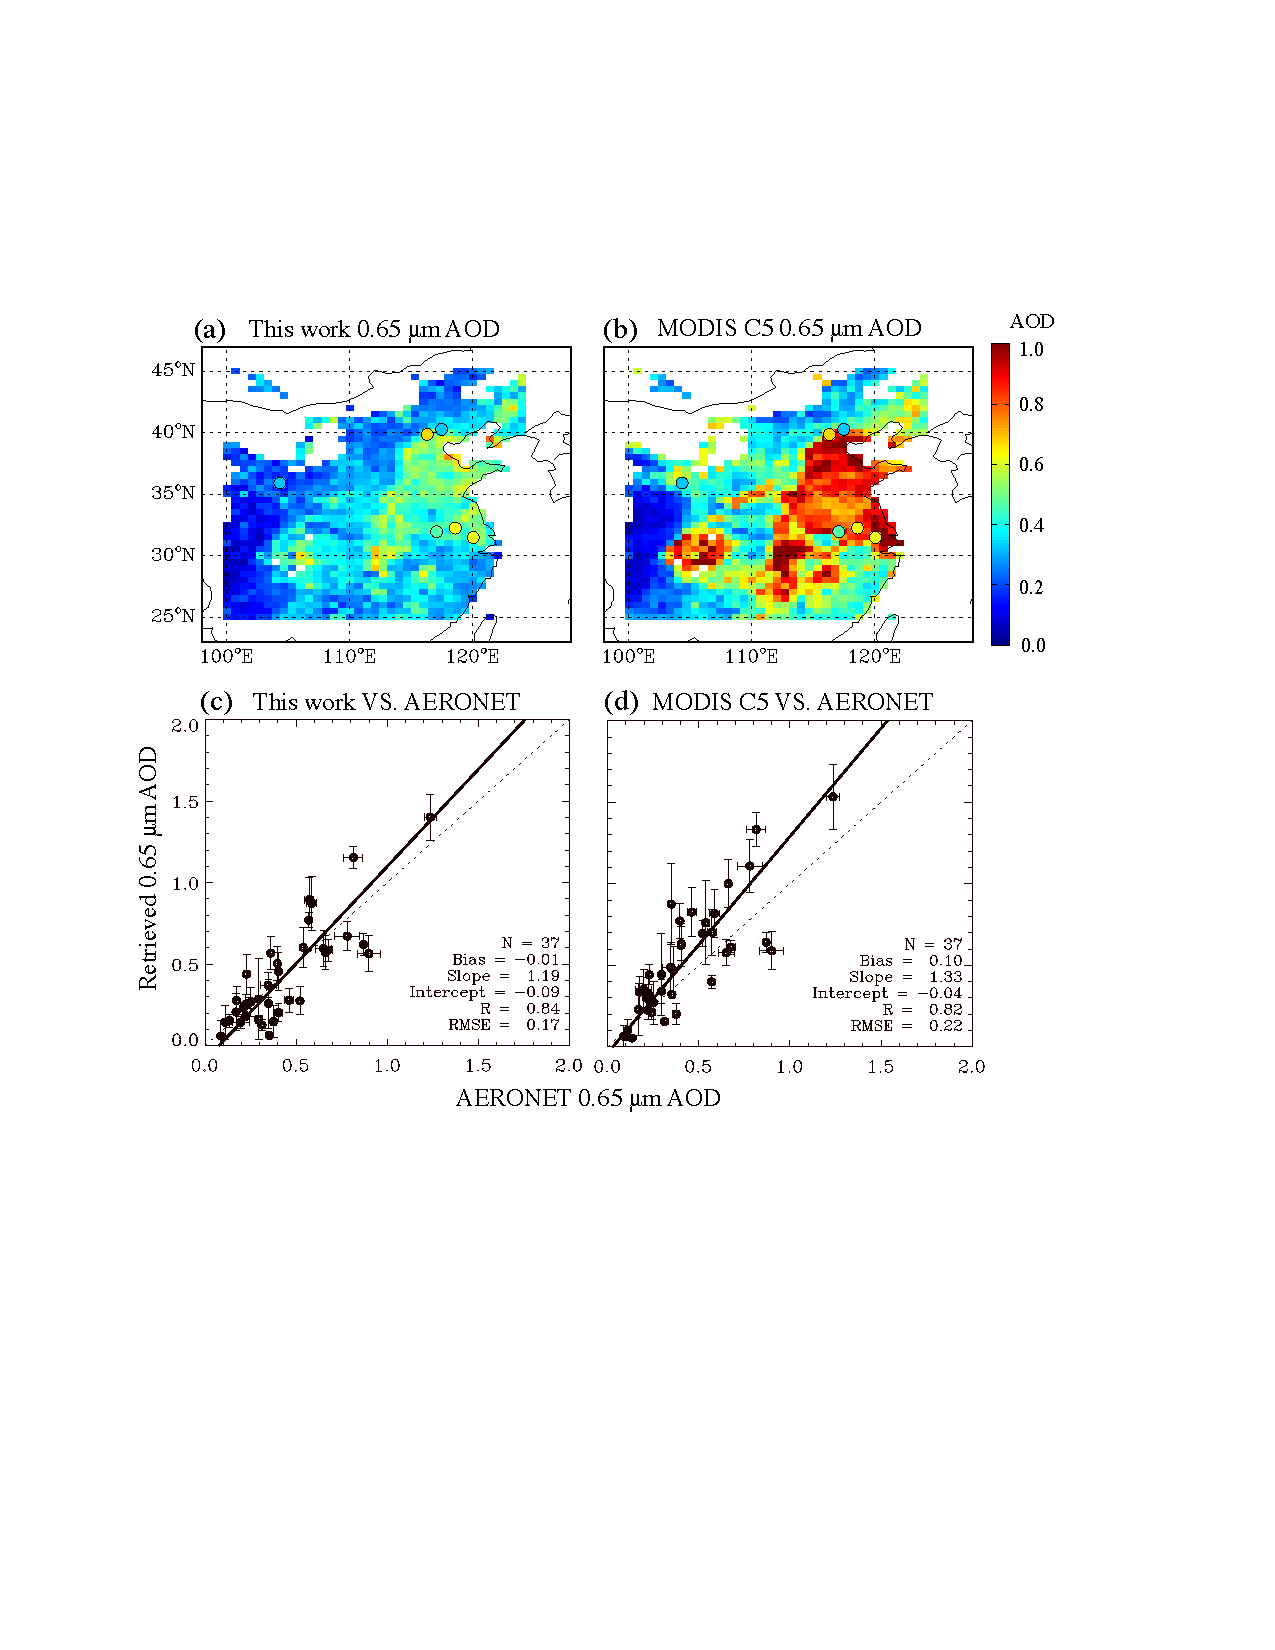
\includegraphics[width={0.8\textwidth}]{figures/a1i.pdf}
  \caption{The 0.65 $\mu$m AOD retrieved by \citep{Wang10} compared with the 
MODIS operational collection 5 AOD products. (a) and (b) are their two-month 
averages for the period of April--May, 2008. The correspondong two-month 
averages of 0.65-$\mu$m AOD collected at size AERONET sites are color-coded 
as circles. (c) and (d) are their scatterplot against AOD observed from 
AERONET sites indicated on the above map. \citep[Figure adopted from][]{Wang10}.}
  \label{fig:modisobs}
 \end{figure}

 GEOS-Chem simulated aerosol composition over Asia is shown by multiple studies 
 to have large underestimation in BC, and equivalent or larger underestimation 
 of OC mass and overestimation of sulfate aerosol mass \citep{Heald05,Fu12},
 which suggests that the mass fraction of highly absorbing (BC) 
 and highly scattering (OC and sulfate) fine mode aerosols may have far less biases 
 (as compared to the relative bias in OC mass only). 
 Consequently, no significant biases are assumed for: 
 (a) the GEOS-Chem simulated fraction of coarse mode (dust) aerosol mass, 
 and (b) the GEOS-Chem simulated aerosol single scattering albedo. 
 While (b) is important to ensure an unbiased retrieval of AOD, 
 (a) supports that the GEOS-Chem simulated dust AOD fraction is likely unbiased, 
 both of which support the use of AOD scale factors derived from MODIS 
 for constraining emission of coarse-mode dust and fine-mode aerosols. 
 Admittedly, any model bias in modeled AOT fraction for each individual species 
 can lead to a corresponding bias (of the same sign) in the adjoint modeling 
 results for individual emission. 
 Quantification of such bias is not possible for the present study 
 owing to the lack of aerosol composition data in China.

%%%\section{Inversion Strategies} \label{sec:invstrategy}

\subsection{Selection of emissions for optimization} \label{subsec:selectems}

 The inversion scheme and the MODIS-based constraints, as described in the preceding sections, 
 are combined to constrain the aerosol emissions over the Eastern Asia 
 for the period of April 2008. 
 The modeled emission parameters that most significantly influence the discrepancy 
 between simulation and observations are selected and spatially constrained. 
 Specifically, those model parameters (or control parameters) represent six emitted tracers, 
 as listed in Table \ref{tab:ems1}, which include emissions of \ce{SO2}, \ce{NH3}, and \ce{NOx}, BC, 
 and OC from anthropogenic sources, and mineral dust. 
 Bottom-up inventories (and an online mobilization scheme for dust) are used as 
 \textit{a priori} estimates, corresponding magnitudes and geographic distributions 
 of which are shown in Table \ref{tab:ems1} and Figure \ref{fig:ems1}, respectively. 
 The temporal extent of the optimization window is selected 
 to be reconcilable with the temporal variability of the bottom-up emission. 
 We set optimization window of a month for those trace gases and carbonaceous emission tracers; 
 while dust emission tracers are constrained daily in a separate optimization run 
 following approach by \citet{Wang12}. 
 Both optimizations assimilate hourly observations during the adjoint simulation. 

 The 4D-Var technique in the optimization requires background 
 error covariance statistics for each control parameter. 
 We specify the priori error for those emission tracers 
 based on characterized spatial and temporal averaged uncertainties for those inventories 
 \citep{Zhang09b,Bond07,Zender03a},
 but with larger values to reflect the possibly large local aerosol emission 
 uncertainties in the bottom-up inventories. 
 The uncertainty for \ce{SO2} emission estimate is believed 
 to be smaller than those for \ce{NH3} and \ce{NOx}, 
 while uncertainties of other tracers could be even larger \citep{Textor06,Zhang09b}.
 Therefore, we set relative error of 50\% for \ce{SO2}, 100\% for \ce{NH3} and NOx, 
 200\% for BC, OC, and dust sources. 
 Lacking information to fully construct a physically representative 
 prior error covariance matrix, a regularization parameter $\gamma$ 
 is introduced in the cost function to balance the contribution of model error
and source error,  with a value (here $\gamma = 1000$) selected using the 
L-curve technique \citep{Hansen98}. Moreover, in order to test the impact of 
those specified uncertainties on the optimization, 
 we run a case with an arbitrary prior error of 100\% for all emission tracers, 
 and present the results in Table \ref{tab:errorsensi}. 

 \subsection{Sensitivity test with pseudo AOD observations} \label{subsec:pseudo}

 We first conduct a pseudo experiment to assess: 
 (1) the concept that temporal variations and geophysical location of AOD, 
 when interpreted with GEOS-Chem model, 
 can yield information about change regarding aerosol composition and emissions, 
 and (2) the sensitivity of the inversion results to the assumption 
 that GEOS-Chem simulated relative composition or single scattering albedo of aerosol is unbiased.
 The experiment has three steps:
 (a) GEOS-Chem simulation with standard bottom-up EIs 
 are first conducted to obtain prior aerosol composition 
 and 0.65 $\mu$m AOD for the period from April 5 to 11 of 2008; 
 (b) Pseudo-observations of AOD are created by perturbing the following emissions 
 (relative to bottom-up EIs) in GEOS-Chem: $+$20\% for \ce{SO2}, \ce{NH3}, and \ce{NOx}, 
 $-$40\% for dust, and zero for BC and OC (Table \ref{tab:pseudo1}); 
 (c) These pseudo-observations of AOD in the dark surface region (red box in Figure \ref{fig:pseudo1}a), 
 twice per day, respectively at the Terra and Aqua overpass daytime, 
 are subsequently used as truth to constrain emissions using the GEOS-Chem adjoint-based inversion. 

 \begin{figure}[t]  \centering  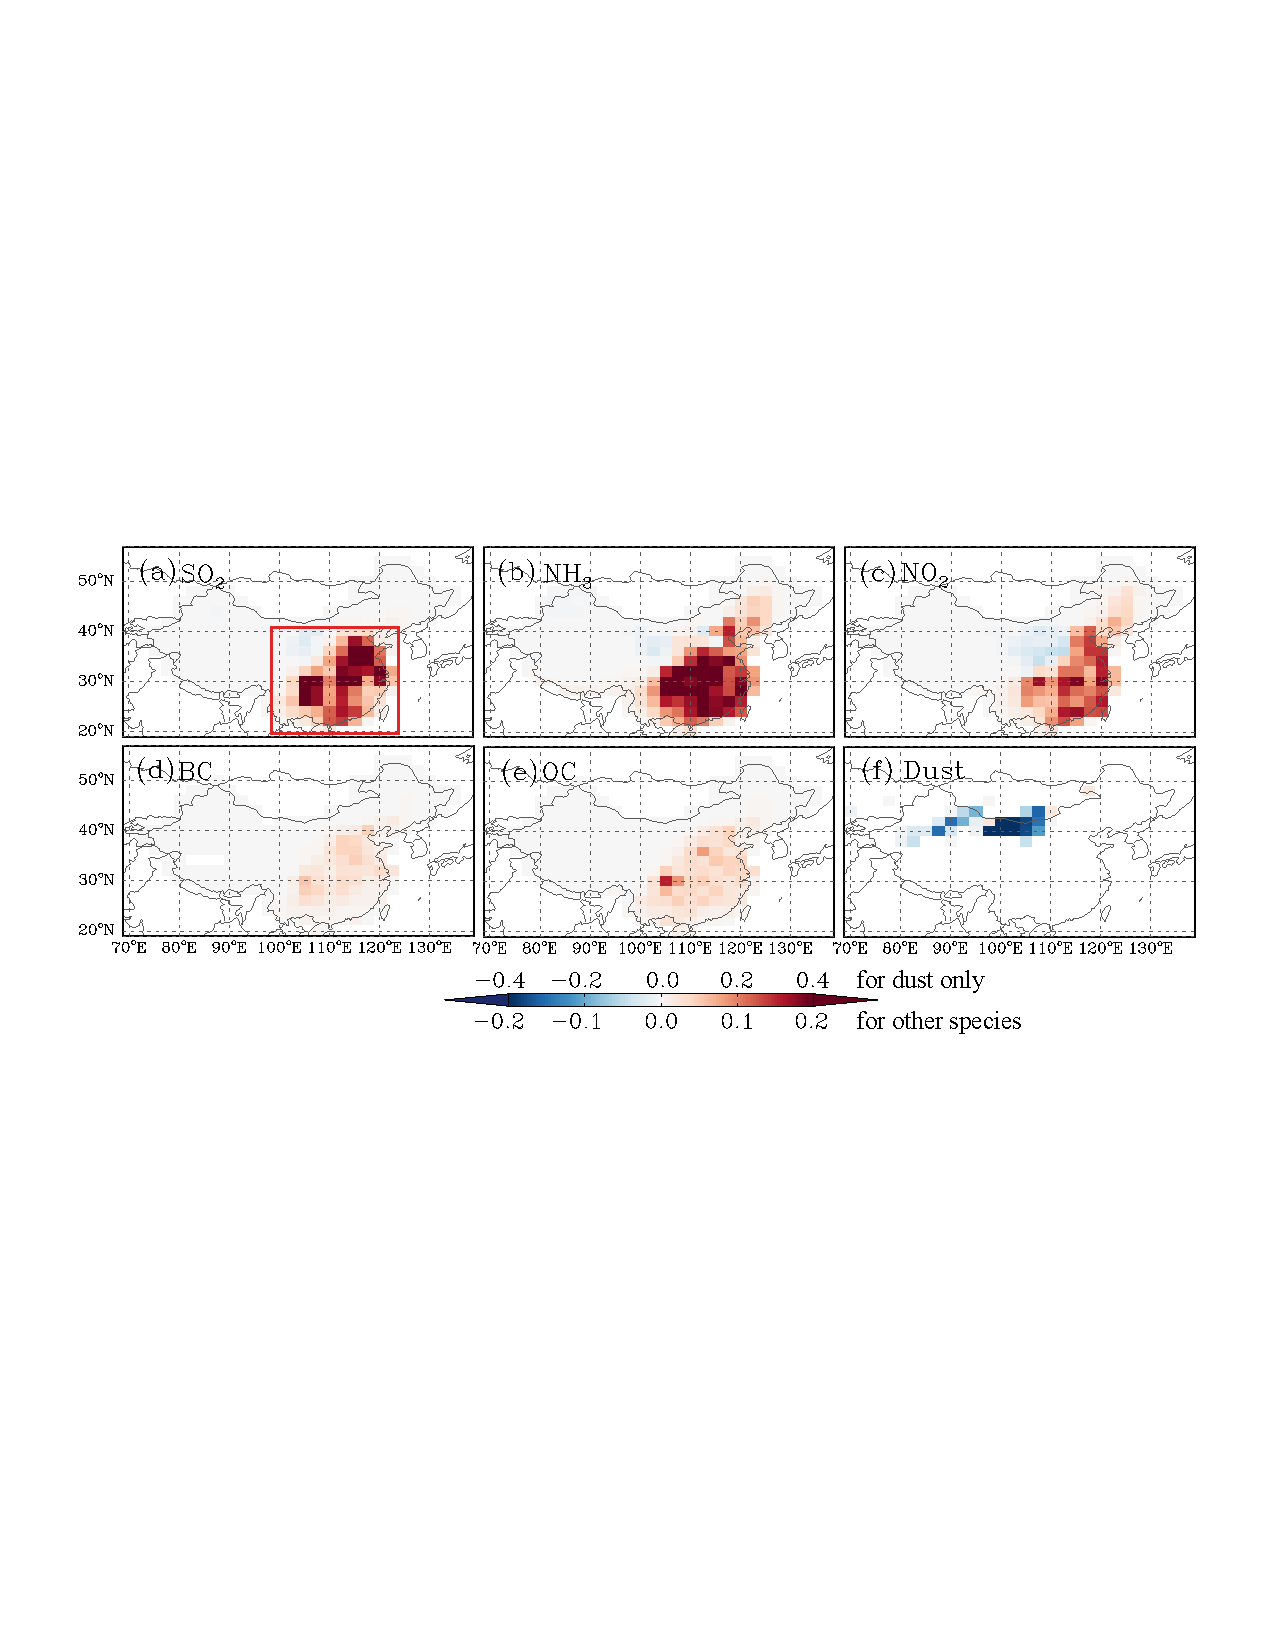
\includegraphics[width={0.95\textwidth}]{figures/a2.pdf}
  \caption{Relative changes in posterior aerosol emissions from \textit{a priori}
   in the pseudo-observation experiment.
   Six panels are respectively for anthropogenic emissions of \ce{SO2}, \ce{NH3},
   \ce{NOx}, BC, and OC, and mineral dust from both natural and anthropogenic sources.
   The red box in panel (a) indicates the region where AOD observations are selected. 
   \citep[Figure adopted from][]{Xu13} }
  \label{fig:pseudo1}
 \end{figure}

 The degree to which the inversion can correct for species-specific errors in the emissions 
 is assessed in these sensitivity tests by comparing the optimized aerosol emissions 
 from (c) can then be evaluated against the truth, or the perturbed emissions in (b).  
 Figure \ref{fig:pseudo1} shows the distribution of relative changes in posterior emissions 
 from the 6th iteration with respect to the prior bottom-up emissions for each species; 
 the overall changes over the China are shown in Table \ref{tab:pseudo1}.
 By the 6th iteration, the cost function reduced by 50\%; 
 further iterations yielded negligible additional decreases. 
 The posterior emissions for \ce{SO2} and \ce{NH3}, which increased by 14\% from the prior, 
 are close to the “truth” (20\%). \ce{NOx} emissions were increased by 8\%, 
 a smaller change than \ce{SO2} and \ce{NH3}. 
 Dust emissions reduced by 26\% percent in the inversion, 
 approaching the true values of $-$40\%.
 BC and OC emissions were increased by 2\% and 3\%, which are close to the truth of 0. 

 Overall, this sensitivity study demonstrates that the inversion is capable of resolving the sign,
 spatial distribution, and the bulk of the true perturbations for the emissions of each species.
 Meanwhile, we also note that the adjoint inversion could transfer (somewhat marginal) errors
 from one tracer to another, such as increases in BC and OC emission 
 as a result of significant underestimations in the prior \ce{SO2}, \ce{NH3}, and \ce{NOx} emissions,
 reflecting errors due to assumptions related to unbiased GEOS-Chem aerosol composition.
 We can also assume that similar aliasing would occur in attempts 
 to distinguish the impacts of co-located precursor emissions of scattering particles
 (e.g., \ce{SO2} and \ce{NOx} from power plants),
 although additional tests would be necessary to assess whether or not differences 
 in the timescales (and thus transported length scales) 
 over which these emissions impact AOD would allow their sources to be separated.
 Long-range transport of dust appears to have less influence on the inversion because:
 (a) except dust, there are little (other) emissions in dust source regions;
 (b) a sudden increase of AOD in downwind regions can be interpreted by GEOS-Chem
 due to the dust transport, and this increase can be used by GEOS-Chem adjoint
  as constraint to optimize the dust emission.

\begin{table}[t]
  \centering
  \small
  \caption{Prior, posterior, and perturbed aerosol emissions over China in the pseudo experiment.}
  \label{tab:pseudo1}
  \begin{tabular}{m{3em} C{5em} C{5em} C{6em} C{6em}}
    \toprule
    Tracer & $E_\text{prior}$ (Gg/Month) & $E_\text{posterior}$ (Gg/Month)& $E_\text{posterior}/E_\text{prior}$ (\%)& $E_\text{perturbed}/E_\text{prior}$ (\%)\\ 
    \midrule
    \ce{SO2} & 520.8 & 592.0 & 113.7 & 120 \\
    \ce{NH3} & 219.3 & 249.2 & 113.7 & 120 \\
    \ce{NOx} & 338.8 & 365.3 & 107.8 & 120 \\
    BC & 23.3 & 23.8 & 102.3 & 100 \\
    OC & 39.7 & 41.1 & 103.4 & 100 \\
    Dust & 2301 & 1697 & 73.7 & 60 \\ 
    \bottomrule
  \end{tabular}
\end{table}

\section{Inversion Results} \label{sec:invresult}

 \begin{figure}[t]
  \centering
  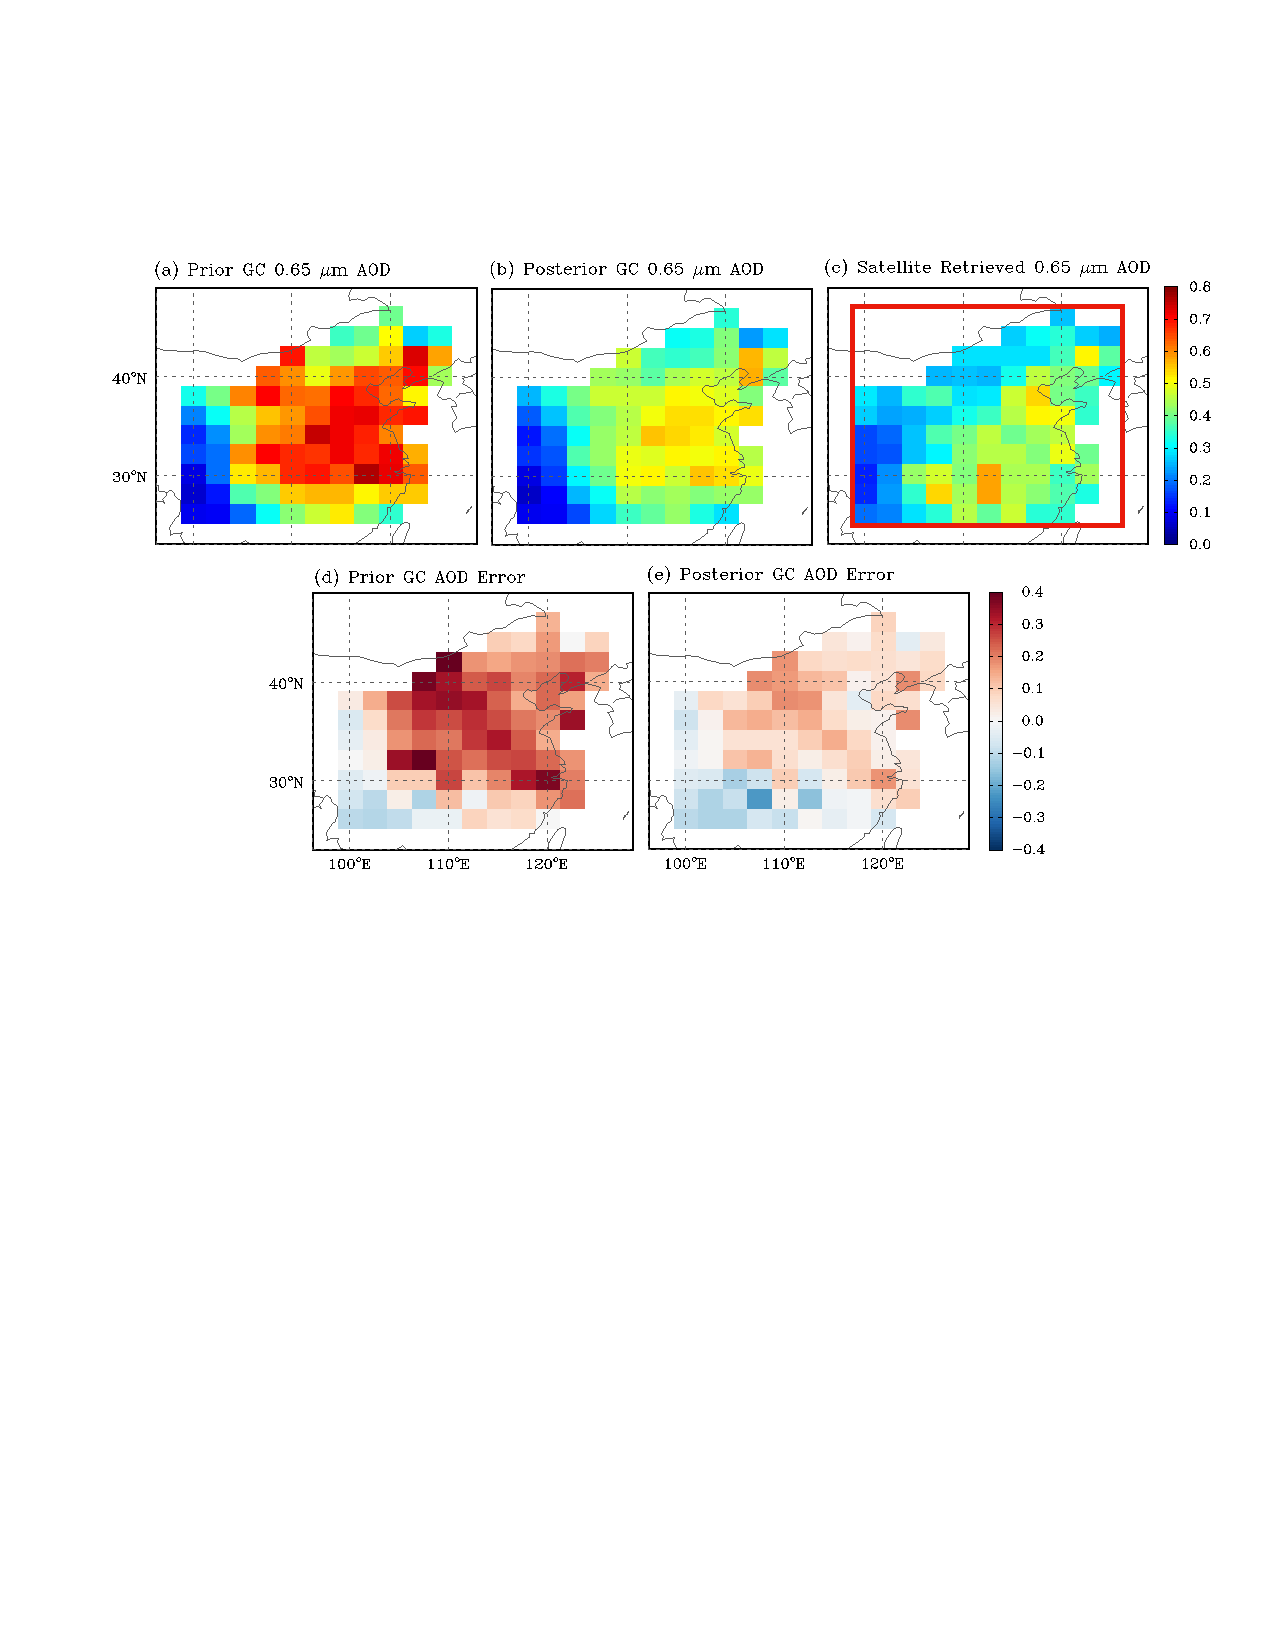
\includegraphics[width={0.95\textwidth}]{figures/a3.pdf}
  \caption{Comparison of the prior (a) and posterior (b) GEOS-Chem (GC) simulation
 of 0.65 $\mu$m AOD with the AOD at the same wavelength retrieved from
 MODIS reflectance using GEOS-Chem aerosol optical properties (c) averaged
 for the period of April 2008. Satellite retrievals with 10 km by 10 km at nadir
 are aggregated to GEOS-Chem grid cells; and the model AOD are sampled coincidentally
 with those retrievals. Panel (d) and (e) respectively show the difference of
 prior and posterior simulated from the satellite retrieved AODs.
 The red box in panel (c) indicates the region where AOD observations are selected.
 \citep[Figure adopted from][]{Xu13}}
  \label{fig:aod1}
 \end{figure}

 With the feasibility of the approach demonstrated in section \ref{subsec:pseudo}, 
 we apply the approach to MODIS radiance data in April 2008. 
 The emissions that result from each iteration during the optimization 
 enable GEOS-Chem to produce a different set of AOD values 
 that converge to the observational constraints. 
 Figure \ref{fig:aod1}a shows the geographic distribution of GEOS-Chem AOD at 0.65 $\mu$m, 
 simulated with prior aerosol emissions, averaged coincidently with retrieved daily MODIS AOD 
 (Figure \ref{fig:aod1}c) during April 2008. 
 While the prior model simulation captures the overall spatial pattern of AOD 
 with larger values over eastern China, 
 it has a slight underestimation over the southwestern China 
 but an overwhelming overestimation elsewhere, 
 when compared to the retrieved AOD from MODIS radiance (Figure \ref{fig:aod1}d). 
 The optimization is expected to adjust aerosol emissions to reduce those differences. 
 Following the experiment design described in section \ref{subsec:selectems}, 
 we find that after 6 iterations of the GEOS-Chem forward and adjoint runs, 
 the cost function is reduced by about 60\%, 
 and further iterations yield negligible reductions in the cost function. 
 Therefore, the aerosol emissions adjusted from the 6th iteration are selected as the final optimal results. 
 As shown in Figure \ref{fig:aod1}b and \ref{fig:aod1}e, the posterior GEOS-Chem AOD 
 that are simulated with the optimized aerosol emissions 
 are in much better agreement with their counterparts retrieved from MODIS reflectance, 
 which is also reflected by the cost function reduction and 
 confirms the effectiveness of the adjustment in top-down emissions.

 %% Figures of the daily variations in the AOD and dust emission
 \begin{figure}[p]
  \centering
  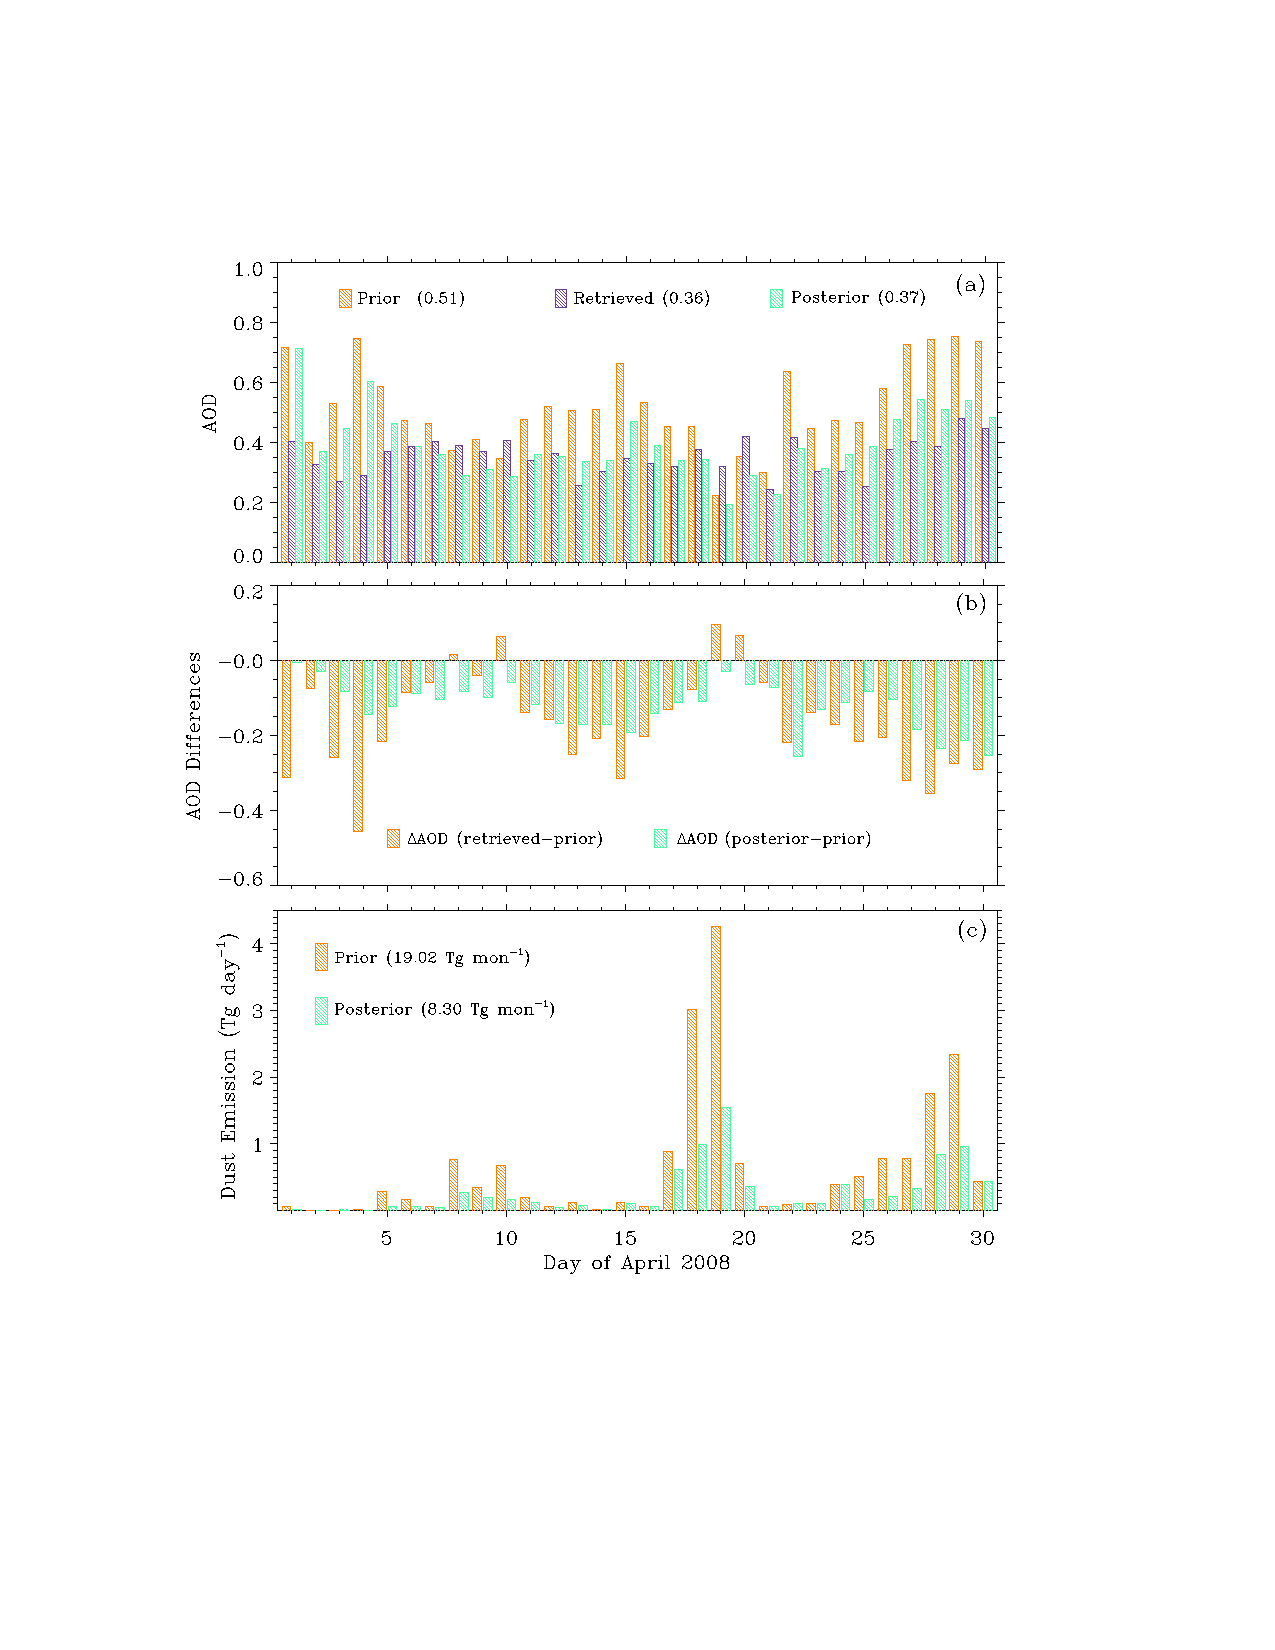
\includegraphics[width={0.8\textwidth}]{figures/a4.pdf}
  \caption{(a) Time series of the spatially averaged daily MODIS AOD
retrievals (purple) for April 2008 over the Eastern China, compared by
the prior (orange) and posterior (green) spatial averaged daily
GEOS-Chem AOD that are sampled in the MODIS AOD tempo-spatial space. (b)
Time series of the expected daily AOD adjustments (orange) that are the
differences between MODIS AOD and the prior GEOS-Chem AOD and their real
adjustments (green) that are the differences of posterior from prior
GEOS-Chem AOD. (c) Time series of the prior (orange) and posterior
(green) daily dust emissions over China for April 2008. \citep[Figure
adopted from][]{Xu13}}
  \label{fig:dailyaod}
 \end{figure}

\begin{table}[t]
  \centering
  \scriptsize
  \caption{List of prior and posterior aerosol emissions in China during April 2008.}
  \label{tab:ems1}
  \begin{tabular}{m{3em} C{4em} C{4em} C{5em} C{3em}
                  C{4em} C{0.1em} C{5em} C{4em} R{3em} }
    \toprule
    \multicolumn{1}{l}{} & \multicolumn{5}{c}{Bottom-Up} & \multicolumn{1}{c}{} & \multicolumn{3}{c}{Top-Down}      \\
    \cline{2-6} \cline{8-10}
    Tracer &  $E_\text{prior}$ (TgMon$^{-1}$) & \textit{a priori} error (\%) & Inventory & Base year & Temporal resolution & & Optimization window & $E_\text{posterior}$ (TgMon$^{-1}$) & ${\Delta}E$ (\%) \\
    \midrule
    \ce{SO2} & 2.60  & 50  & INTEX-B & 2006   & Annual  & & Monthly & 1.73 & $-$33.5 \\
    \ce{NH3} & 1.10  & 100 & INTEX-B & 2000   & Annual  & & Monthly & 0.72 & $-$34.5 \\ 
    \ce{NOx} & 1.69  & 100 & INTEX-B & 2006   & Monthly & & Monthly & 1.38 & $-$18.8 \\
    BC       & 0.11  & 200 & Bond07  & 2000   & Monthly & & Monthly & 0.10 & $-$9.1  \\ 
    OC       & 0.21  & 200 & Bond07  & 2000   & Monthly & & Monthly & 0.18 & $-$15.0 \\
    Dust     & 19.02 & 200 & DEAD    & Online & Hourly  & & Daily   & 8.30 & $-$56.4 \\
    \bottomrule
  \end{tabular}
\end{table}

 The convergence of the model simulation to the MODIS AOD retrievals 
 is also indicated in the AOD daily variability. 
 Figure \ref{fig:dailyaod}a shows the daily variations of the AOD 
 spatially averaged for available MODIS retrievals (purple) over the eastern China areas 
 within the red box in Figure \ref{fig:aod1}c, and the coincidental GEOS-Chem simulation
 prior and posterior to the aerosol emission optimization (orange and green, receptively).
 The prior model produce overestimated AODs for most days during the month.
 After top-down adjustments to the aerosol emissions,
 such overestimation of the AOD is reduced in total over the course of the month.
 As shown in Figure \ref{fig:dailyaod}b, the real changes of the modeled daily AOD 
 during the optimization (green bars), or equivalently, the differences of the posterior
 from the prior are consistent with the expected changes, i.e.,
 the differences of the MODIS retrievals from the prior model simulation.
 It is noted that the posterior AODs has larger departure from the observation
 than the prior on a few days.
 This reflects that monthly-scaled emissions are not perfectly capturing the daily variation of emission.

 %% Figures of the optimized ems
 \begin{figure}[p]
  \centering
  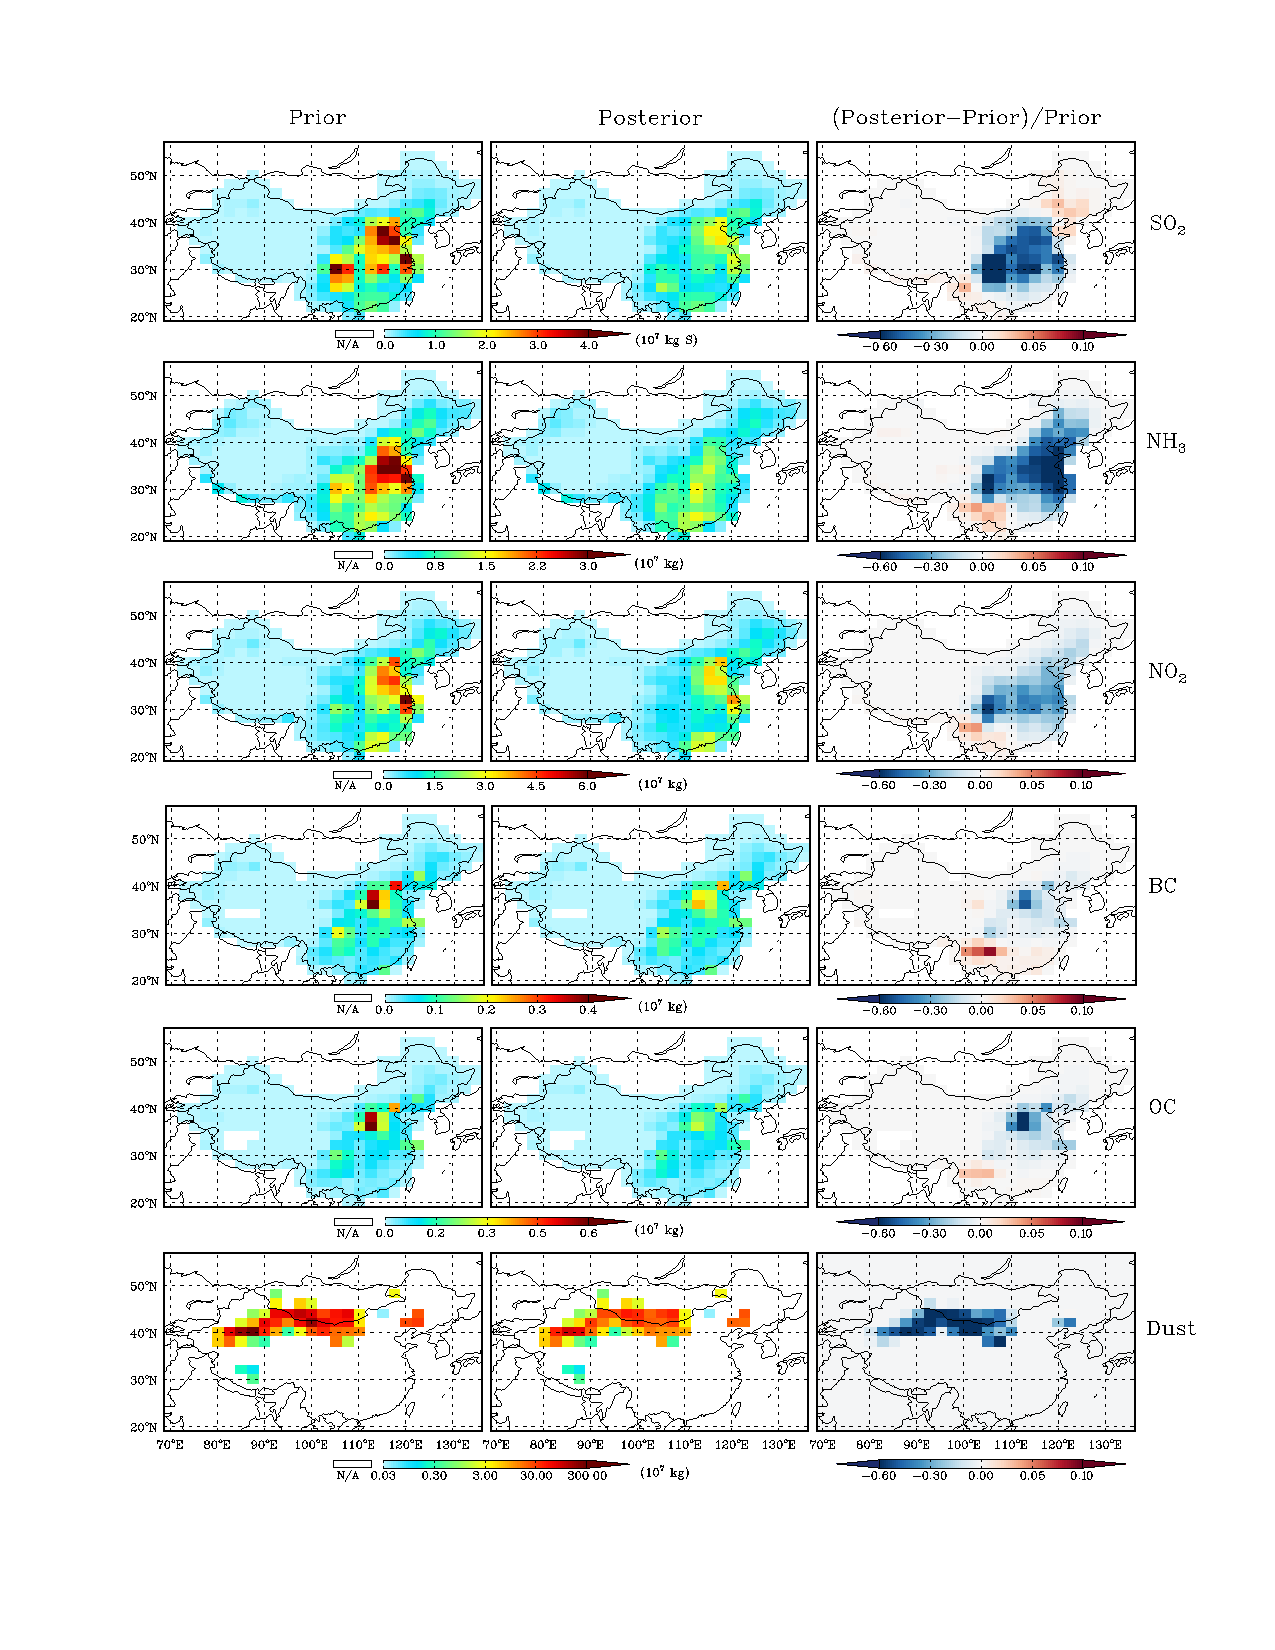
\includegraphics[width={0.95\textwidth}]{figures/a5.pdf}
  \caption{The prior (or bottom-up based, left column), optimized (or
top-down constrained, middle column) aerosol emissions over China for
the period of April 2008, and their relative differences (right column).
Six rows from top to bottom are respectively for anthropogenic emissions
of \ce{SO2}, \ce{NH3}, ce{NOx}, BC, and OC, and mineral dust from both
natural and anthropogenic sources. \citep[Figure adopted from][]{Xu13}}
  \label{fig:ems1}
 \end{figure}

 Emissions of \ce{SO2}, \ce{NH3}, \ce{NOx}, BC, and OC from anthropogenic sources
 are optimized monthly and rescaled over each individual
 2$^{\circ}$ by 2.5$^{\circ}$ grid cell of China for the month of April 2008.
 The prior and posterior (optimized) emissions of these tracers
 are respectively shown in left and middle columns of Figure \ref{fig:ems1},
 in which the relative changes of these emissions in the optimization
 are also included in the right column. Overall, the optimization yields
 an overwhelming reduction for all emission tracers,
 even though some local increases are found.
 As expected, such adjustment in the constrained aerosol emissions
 is consistent with the changes in GEOS-Chem AOD before and after optimization,
 as aerosol loadings usually positively respond to the aerosol emissions.
 Quantitatively, anthropogenic emissions over China continent for the study period
 are changed by $-$33.5\% for \ce{SO2} from 1.302 to 0.866 Tg, $-$34.5\% for \ce{NH3} from 1.096 to 0.718 Tg,
 $-$18.8\% for \ce{NOx} from 1.694 to 1.375 Tg, $-$9.1\% for BC from 0.11 to 0.10 Tg,
 and $-$15.0\% for OC from 0.205 to 0.175 Tg (see Table \ref{tab:ems1}).
 The largest reduction occurs sharply in the central regions of the Eastern China,
 corresponding to the region where the largest AOD are adjusted to the MODIS retrievals.
 Small increases of emitted anthropogenic sources of gases and carbonaceous particles
 are found over the southwestern China, which can be explained
 as the response for the underestimation of AOD in the model simulation over these regions
 (Figure \ref{fig:aod1}a, d). 

 The mineral dust emissions from both anthropogenic and natural sources are optimized daily.
 The adjoint has no leverage to increase the dust emissions over grid cells
 having zero dust emission in the priori estimate identified by the modified DEAD scheme.
 Thus, the posteriori dust source region remains un-shifted as shown
 in Figure \ref{fig:ems1} (bottom panels), which is reasonable
 because the expansion or shrinkage of desert regions is unlikely to extend beyond
 the grid size (2$^{\circ}$ by 2.5$^{\circ}$) of this study \citep{Zender03a,Fairlie07}.
 The total amount of the optimized dust emissions for April 2008 over China is 8.3 Tg,
 reduced by 56.4\% from the modified DEAD module simulation of 19.02 Tg.
 Such reduction indicates an overestimation in the prior emissions of dust,
 especially over Gobi deserts that are located in the Northwestern China and the southern Mongolia.
 \citet{Wang12} presented a similar result,
 but only for a dust event that occurred in the later portion of our study time period.
 Figure \ref{fig:dailyaod}c illustrates the time series of the prior and optimized
 daily total dust emission.
 Two sharp peaks of the dust emissions indicate the occurrences of strong dust storms
 after April 15. Such large temporal variation in the daily scale
 requires the optimization of dust emission on the daily basis. 

 An additional case with specified error of 100\% for all the anthropogenic emission tracers
 is conducted to examine the sensitivity of those specified error to the optimization.
 Table \ref{tab:errorsensi} shows the relative change in optimized emissions for two different scenarios.
 Less than 0.5\% of difference in the optimized emissions is found,
 which means the uncertainty in a priori emission could have
 much smaller impact on the optimization than the observational constraints.

\begin{table}[t]
  \centering
  \small
  \caption{Test of the sensitivity of optimization with respect to prescribed a priori error.}
  \label{tab:errorsensi}
  \begin{tabular}{m{3em} C{4em} C{3em} C{0.1em} C{4em} C{3em} }
    \toprule
    \multicolumn{1}{l}{} & \multicolumn{2}{c}{Case 1} & \multicolumn{1}{c}{} & \multicolumn{2}{c}{Case 2}      \\
    \cline{2-3} \cline{5-6}
    Tracer &  \textit{a priori} error (\%) & ${\Delta}E$ (\%) & & \textit{a priori} error (\%) & ${\Delta}E$ (\%) \\
    \midrule
    \ce{SO2} & 50  & $-$33.5 & & 100 & $-$33.7  \\
    \ce{NH3} & 100 & $-$34.5 & & 100 & $-$34.4  \\
    \ce{NOx} & 100 & $-$18.8 & & 100 & $-$18.8  \\
    BC       & 200 & $-$9.1  & & 100 & $-$9.1   \\
    OC       & 200 & $-$15.0 & & 100 & $-$15.0  \\
    \bottomrule
  \end{tabular}
\end{table}

\section{Results Evaluations}  \label{sec:invevaluation}

 Because direct measurements of the aerosol emissions are few over China,
 we assess the optimized sources by comparing the GEOS-Chem posterior
 simulated aerosol mass concentrations and AOD with
 the independent observations from various sources.
 The evaluation datasets include:
 (1) AERONET AOD observations \citep{Holben98} over nine sites;
 (2) Level 3 MISR daily AOD products \citep{Kahn05,Martonchik09};
 (3) Level 3 \ce{SO2} \citep{Krotkov06,Lee09}
 and Level 2 \ce{NO2} \citep{Bucsela06} retrievals from the Ozone Monitoring Instrument (OMI);
 (4) surface mass concentration of sulfate-nitrate-ammonium (SNA) aerosol particles over Qingdao, China;
 and (5) surface PM\textsubscript{10} over two sites close to dust source region \citep{Ge10}. 

 \subsection{Comparison with AERONET AOD}

 We first evaluate the prior and posteriori GEOS-Chem 0.55 $\mu$m AOD against
 the AERONET AOD at 0.55 $\mu$m that are interpolated from AODs at 0.44 and 0.67 $\mu$m
 based on the Angstrom exponent.
 Three-hour averaged values of available AERONET AOD,
 centered by the model output time are used to compare with
 the model AOD over the grid cells locating the AERONET sites.
 The scatterplots shown in Figure \ref{fig:aeronet} are the comparisons
 for nine stations over China, South Korea, and Japan representing different aerosol types.
 The first three stations, i.e., (a) Zhangye, (b) SACOL, and (c) Jingtai,
 which are located over rural regions in the south boundary of Gobi deserts
 and have little influence from anthropogenic emissions,
 are representative sites for dust aerosol \citep{Ge10}.
 The next three sites, (d) Beijing, (e) Xinglong, and (f) Heifei,
 are located in anthropogenic source regions.
 The last three sites, (g) Noto, (h) Shirahama, and (i) Gwangju\_K,
 are located over Japan and South Korea, the downwind regions of China emissions.
 Those last six stations are affected not only by the local anthropogenic emissions
 but also by the long-range transported aerosols from the upwind regions.
 Indeed, those three categories of stations are respectively located
 in the upwind, central, and downwind of regions having the observational constraints.

 %% Validation vs AEORNET
 \begin{figure}[t]
  \centering
  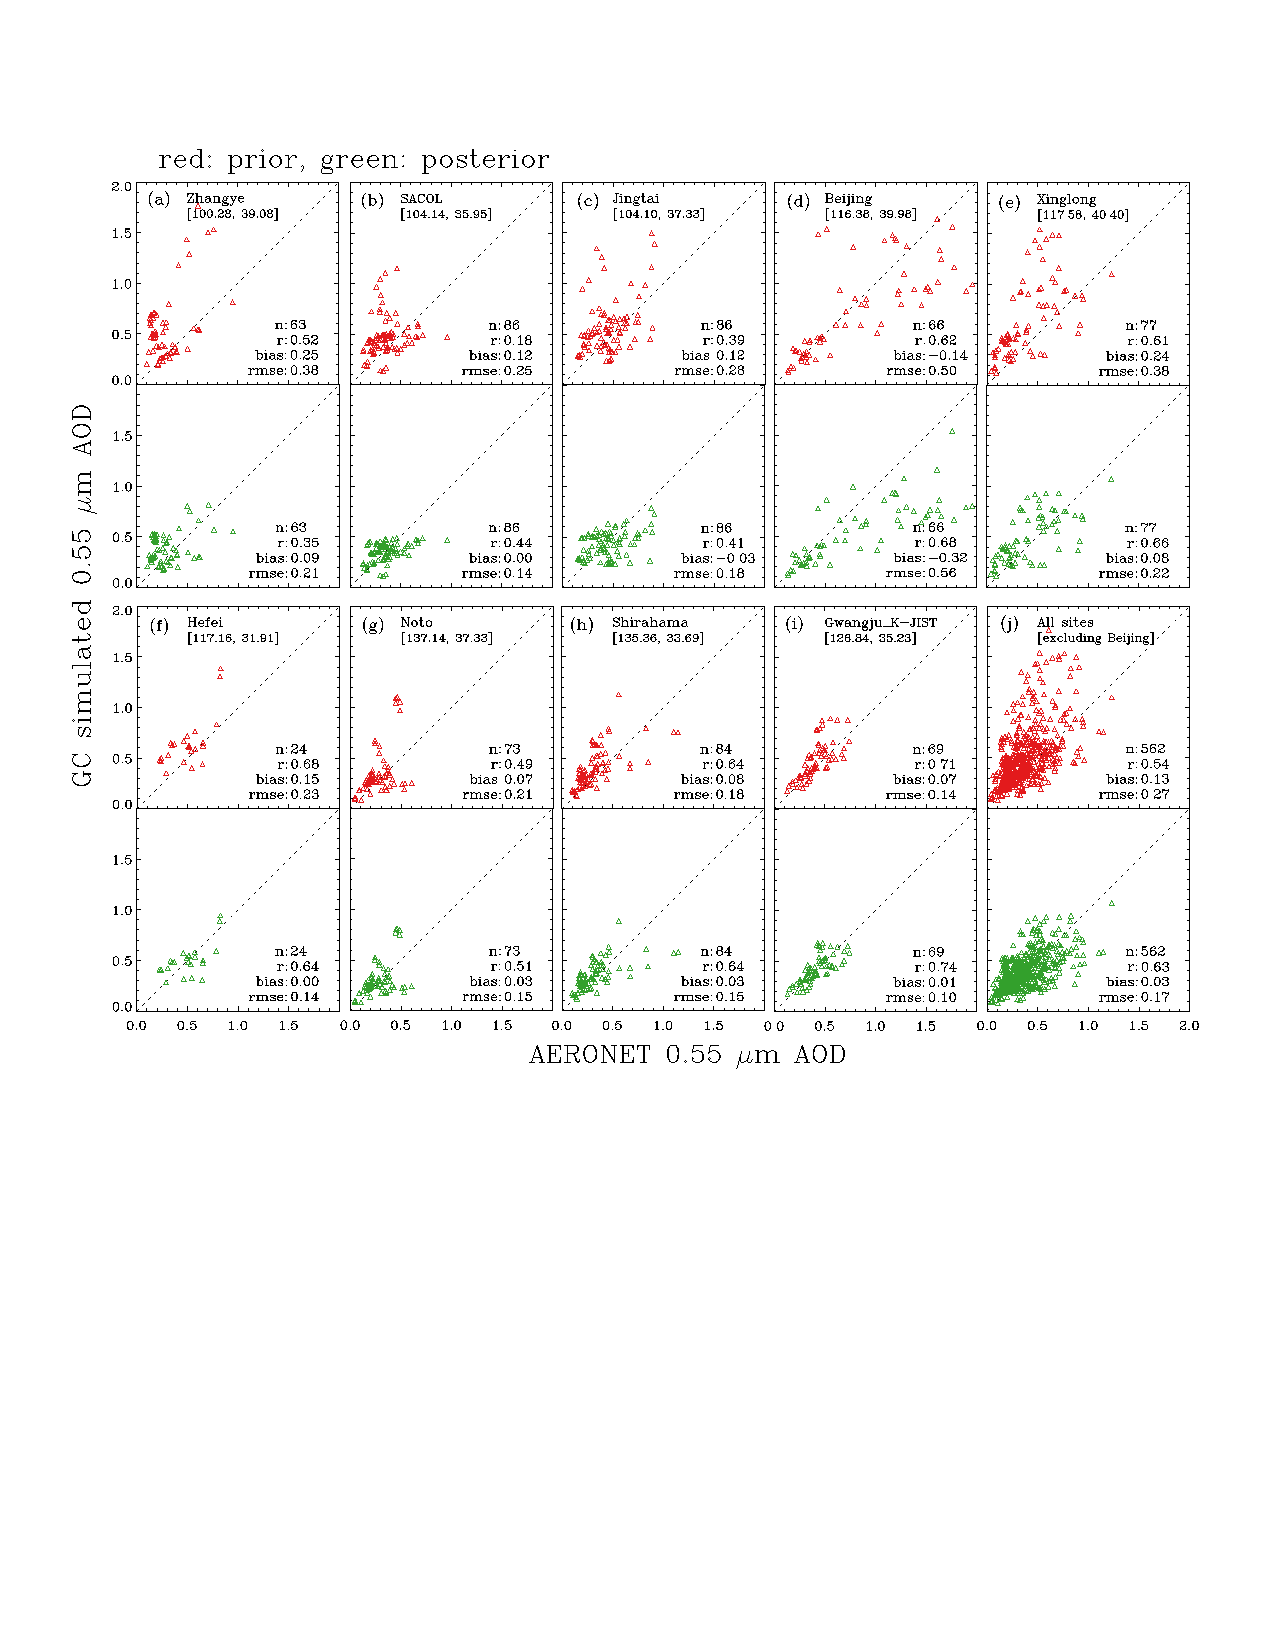
\includegraphics[width={0.99\textwidth}]{figures/a6.pdf}  
  \caption{(a – i) Scatterplots of GEOS-Chem AOD versus AERONET AOD at 0.55 $\mu$m prior (red scatters) and posterior (green scatters) to the aerosol emission optimization over nine stations. AERONET AODs are 3-hour averages following the GEOS-Chem output frequency. (j) The overall comparison for eight AERONET sites excluding Beijing. Also shown are the number of valid sampled pairs (n), correlation coefficients (R), bias, and root-mean-square-error (rmse).}
  \label{fig:aeronet}
 \end{figure}

 The prior GEOS-Chem simulation (shown in the red scatter panels)
 overestimates the AERONET AOD for all the sites except Beijing.
 The negative bias of model AOD at Beijing is likely owing to the model coarse resolution,
 which fails to resolve heavy local urban pollution.
 The geographic area of urban Beijing is about 1300 km\textsuperscript{2}
 (\url{http://en.wikipedia.org/wiki/Beijing}),
 less than 3\% of the area of a GEOS-Chem grid cell.
 Thus, the local pollution signal is smeared in the model grid box.
 Moreover, Beijing and Xinglong are in the same model grid cell,
 but AERONET AOD over Xinglong is much smaller than that over Beijing site
 (as later shown as circles on the maps of Figure \ref{fig:misr1}a-c).
 As Beijing site is difficult to represent in the GEOS-Chem at 2$^{\circ}$ by 2.5$^{\circ}$ resolution,
 we exclude Beijing site in our further analysis.
 GEOS-Chem AOD from the posterior aerosol emissions are in more agreement with the AERONET AOD
 (shown in the green scatter panels),
 as indicated by reduced bias and root-mean-square-error (rmse) over all the other sites and
 increased correlation coefficients (R) for most sites.
 The overall comparison (Figure \ref{fig:aeronet}j) shows the correlation coefficient
 increases from 0.54 to 0.63, and the bias (rmse) declines from 0.13 (0.27) to 0.03 (0.07). 

 \subsection{Comparison with MISR AOD }

 We re-grid the Level 3 daily MISR 0.55 $\mu$m AOD from the 0.5$^{\circ}$ by 0.5$^{\circ}$
 resolution to GEOS-Chem 2$^{\circ}$ by 2.5$^{\circ}$ grid cells and take monthly average for April 2008,
 the geographic distribution of which are shown in Figure \ref{fig:misr1}c.
 High AOD values are found over the eastern China and the northwestern desert regions,
 which are associated to the anthropogenic pollution primarily from
 the industry and wind-blown mineral dust, respectively.
 The monthly sun-photometer AOD values at the same wavelength show
 good agreements with the MISR AOD over all the AERONET sites
 except Beijing where the significant local urban pollution exists.

 %% Validation against MISR
 \begin{figure}[t]
  \centering
  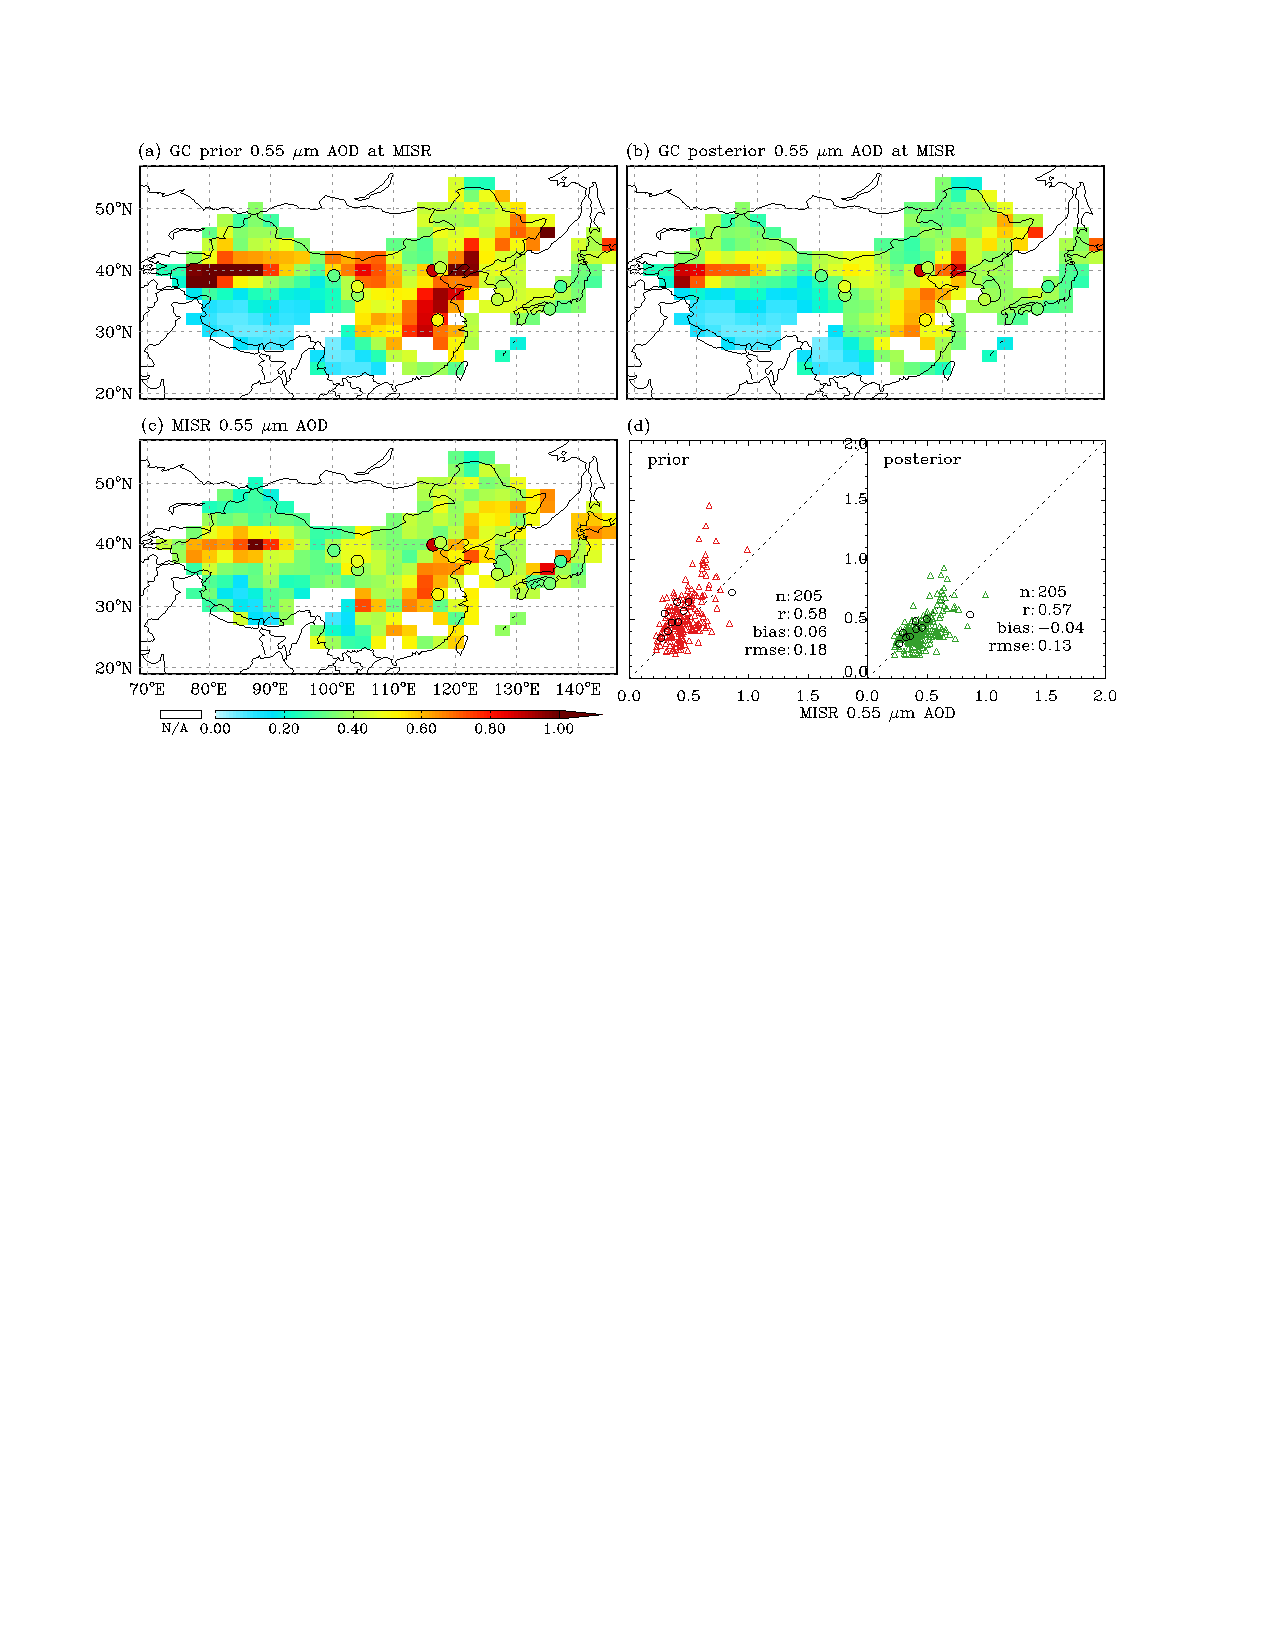
\includegraphics[width={0.9\textwidth}]{figures/a7.pdf}  
  \caption{Comparison of the prior and posterior GEOS-Chem simulation of
0.55 $\mu$m AOD with the level 3 MISR 0.55 $\mu$m AOD for the period
April 2008. (a) The prior GEOS-Chem 0.55 $\mu$ AOD that are sampled
coincidentally with MISR AODs for the period of April 2008. Also
overlaid circles are the monthly AOD averages at 0.55 $\mu$m observed
from the nine AEORNET sites shown in Figure \ref{fig:aeronet}. (b) Same
as (a) but for the monthly average of posterior GEOS-Chem AOD. (c)
Monthly average of the Level 3 daily MISR 0.55 $\mu$m AOD.  (d) Scatter
plot the GEOS-Chem AOD versus the MISR AOD before (red scatters) and
after optimization (green scatters), in which each point indicates an
AOD pair over a model grid cell with value over 0.2. Also shown are the
statistics including number of sampled pairs (n), correlation
coefficient (R), bias and root-mean-square-error (rmse). Comparisons of
the monthly GEOS-Chem AOD versus AERONET AOD are also included as the
black circles; each circle indicates an AOD pair over an individual
site. \citep[Figure adopted from][]{Xu13}}
  \label{fig:misr1}
 \end{figure}

 The monthly averages of prior and posterior GEOS-Chem 0.55 $\mu$m AOD
 mapped in Figure \ref{fig:misr1}a--b are sampled coincidently to the MISR AOD.
 A comparison with the MISR AOD shows GEOS-Chem simulation with prior aerosol emissions
 overestimates AOD over both the desert and industrial regions.
 The posterior simulation is slightly more in agreement with MISR AOD.
 To facilitate the comparison of model with MISR AOD, we also include, as Figure \ref{fig:misr1}d,
 the scatterplots of the AOD for each GEOS-Chem grid cell with values larger than 0.2
 by considering the larger retrieval uncertainty in the low AOD conditions \citep{Kahn05,Kahn10}.
 While the correlation coefficients remain about the same,
 both absolute bias and rmse are reduced about 30\%.

 \subsection{Comparisons with OMI columnar SO\textsubscript{2} and NO\textsubscript{2}}

 The improvement in the optimized aerosol emissions is also exhibited
 in the comparison of simulated trace gases to the satellite retrievals from OMI.
 The GEOS-Chem \ce{SO2} simulations are assessed with OMI Level 3 daily products
 of planetary boundary layer (PBL) \ce{SO2} column gridded
 with 0.25$^{\circ}$ by 0.25$^{\circ}$ resolution.
 We average the OMI \ce{SO2} columnar retrievals into GEOS-Chem 2$^{\circ}$ by 2.5$^{\circ}$ grid cells
 and take the monthly average for comparison, which are shown in Figure \ref{fig:omso2}c.
 Figure \ref{fig:omso2}a and \ref{fig:omso2}b show model prior and posterior \ce{SO2} column
 that are coincidentally sampled with OMI retrievals.
 Figure \ref{fig:omso2}d illustrates the quantitative analysis for OMI \ce{SO2} retrievals
 larger than $1.0 \times 10^{16}$ molec cm$^{-2}$.
 With the optimized emission estimates, the bias and RMSE are reduced
 from 0.81 and 0.61 to --0.28 and 0.38 ($\times 10^{16}$ molec cm$^{-2}$), respectively,
 along with an increase of correlation coefficient from 0.68 to 0.73. 

 %% Validation against OMI SO2
 \begin{figure}[t]
  \centering
  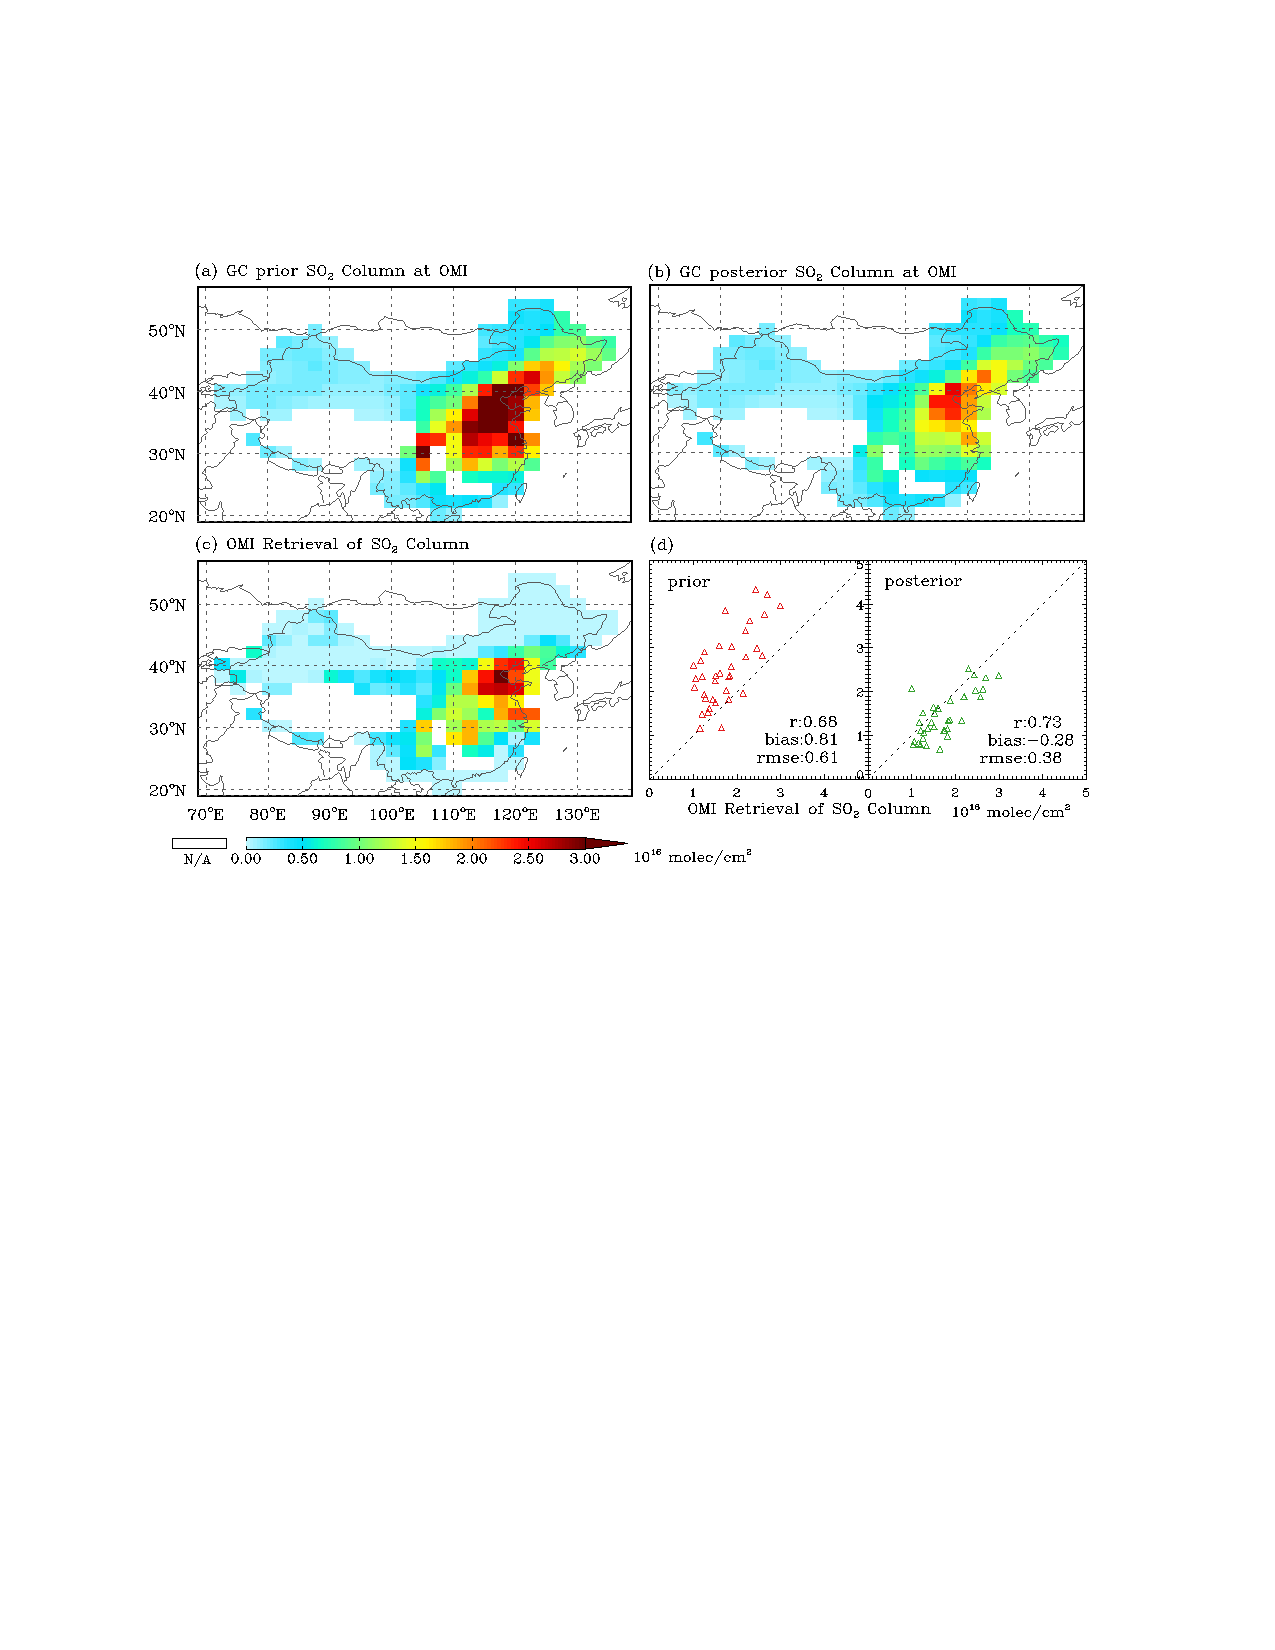
\includegraphics[width={0.9\textwidth}]{figures/a8.pdf}
  \caption{Same as figure \ref{fig:misr1} but for comparison of the GEOS-Chem \ce{SO2} simulation with OMI column \ce{SO2} retrievals for the period of April 2008. The OMI planetary boundary layer (PBL) column \ce{SO2} from the Level 3 daily products with 0.25$^{\circ}$ by 0.25$^{\circ}$ resolutions are aggregated into GEOS-Chem grid cells.}
  \label{fig:omso2}
 \end{figure}

 %% Validation against OMI NO2
 \begin{figure}[t]
  \centering
  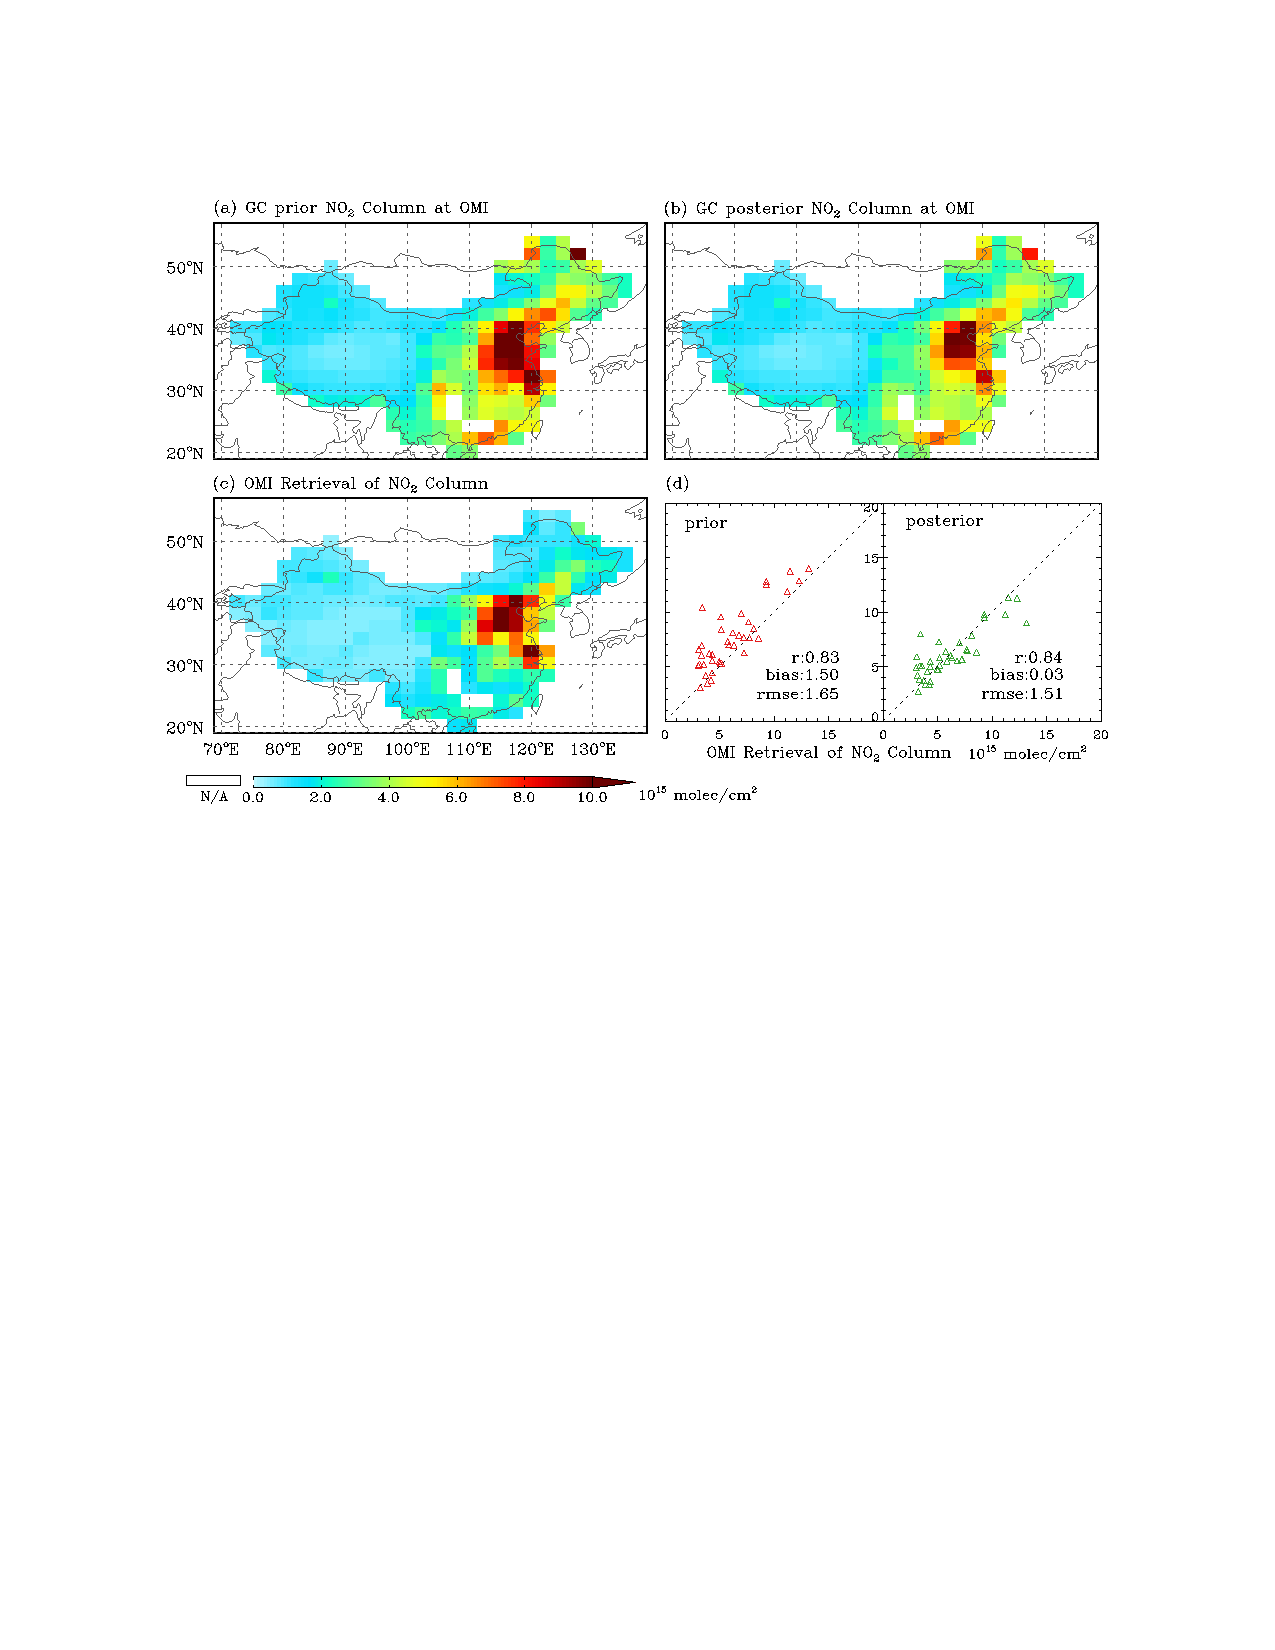
\includegraphics[width={0.9\textwidth}]{figures/a9.pdf}
  \caption{Same figure \ref{fig:misr1} but for comparison of the GEOS-Chem \ce{NO2} simulation with OMI column \ce{NO2} retrievals for the period of April 2008.  The OMI tropospheric column \ce{NO2} from Level 2 daily products with 0.25$^{\circ}$ by 0.25$^{\circ}$ resolutions are aggregated into GEOS-Chem grid cells.}
  \label{fig:omno2}
 \end{figure}

 We evaluate the model simulation of \ce{NO2} with OMI Level 2 products of
 \ce{NO2} tropospheric column over 0.25$^{\circ}$ by 0.25$^{\circ}$ grid cells.
 Recent studies suggested that the uncertainty in OMI \ce{NO2} tropospheric column retrievals
 is about 40\% with an about 15\% positive systematical bias \citep{Boersma08,Celarier08}.
 Following \citet{Lin10}, we apply a factor of 0.85 to OMI \ce{NO2} retrievals
 in our comparison to correct the bias.
 Figure \ref{fig:omno2} shows the comparison of GEOS-Chem \ce{NO2} columns
 with re-gridded OMI \ce{NO2} retrievals.
 Similarly, we also perform the quantitative analysis, as in Figure \ref{fig:omno2}d,
 for OMI \ce{NO2} column retrievals larger than $3.0 \times 10^{15}$ molec cm$^{-2}$.
 While the correlation coefficient remains about the same, the bias (RMSE) is reduced
 from 1.50 (1.65) to 0.03 (1.51) (units: $10^{15}$ molec cm$^{-2}$) after constraining aerosol emissions. 

 \subsection{Comparisons with near-surface aerosol mass concentrations}

 The accuracy of the sulfate-nitrate-ammonium (SNA) aerosol simulation
 is in part determined by the representation of the emissions of \ce{SO2} and \ce{NOx} and \ce{NH3},
 and hence GEOS-Chem simulations with constrained emissions should
 provide overall an improved simulation of SNA.
 Figure \ref{fig:sna} shows the comparison of daily near-surface SNA mass concentration
 from the prior and posterior GEOS-Chem simulations with measurements
 over Qingdao (120.34$^{\circ}$ E, 36.06$^{\circ}$ N), China.
 The error bars for the GEOS-Chem curves indicate the diurnal standard deviation.
 An overestimation in the prior model surface SNA simulations is found
 when comparing with observed counterparts, which shows a bias of 14.28 $\mu$g m$^{-3}$,
 RMSE of 21.84 $\mu$g m$^{-3}$, and correlation coefficient of 0.46.
 Such bias is significantly reduced to 0.34 $\mu$g m$^{-3}$
 in the simulation with top-down constrained emissions,
 along with a 50\% decrease in RMSE and a 28\% increase in correlation coefficient.

 %% Validation against surface SNA
 \begin{figure}[ht]
  \centering
  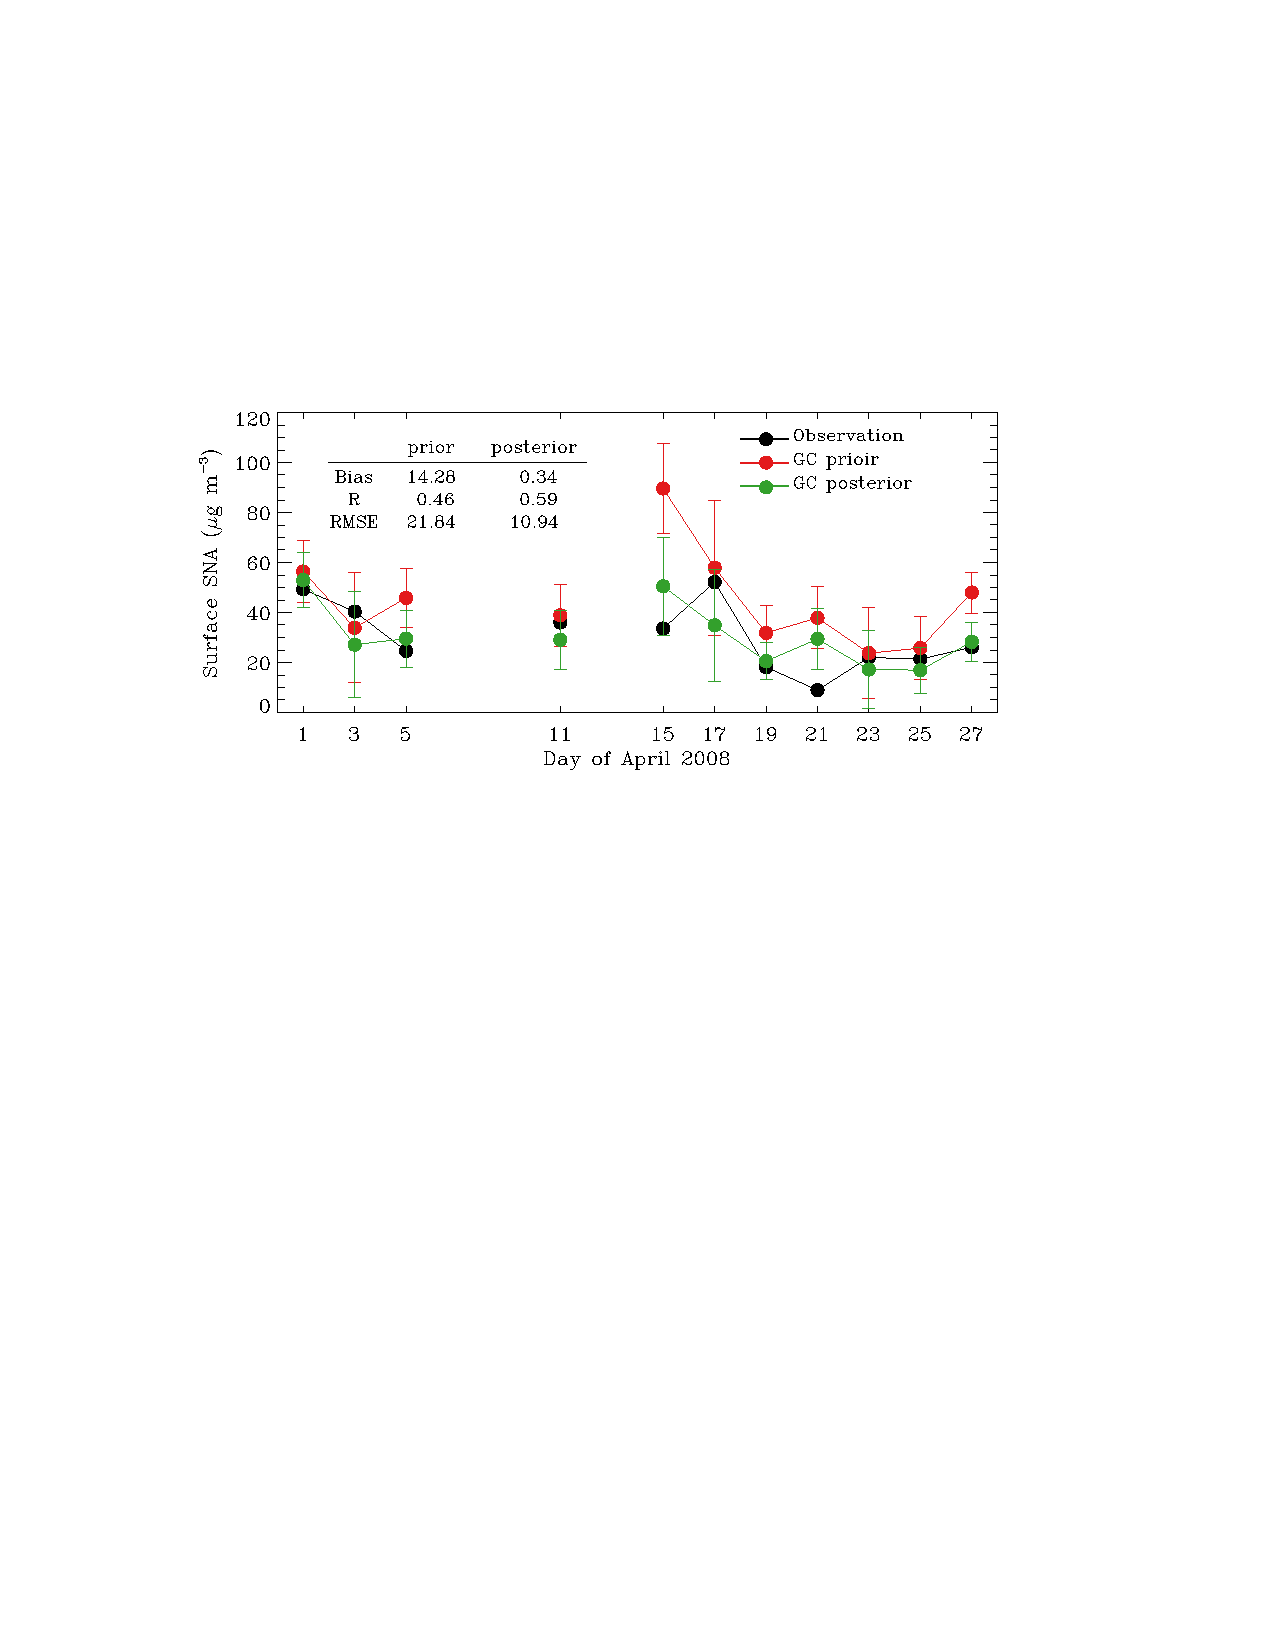
\includegraphics[width={0.8\textwidth}]{figures/a10.pdf}
  \caption{Comparison of the GEOS-Chem surface mass concentration of sulfate-nitrate-ammonium (SNA) aerosols with ground-based observations over Qingdao (120.34$^{\circ}$ E, 36.06$^{\circ}$ N), China. Discontinuity in time series is due to missing or quality filtered observations.}
  \label{fig:sna}
 \end{figure}

 %% Validation against surface PM10
 \begin{figure}[t]
  \centering
  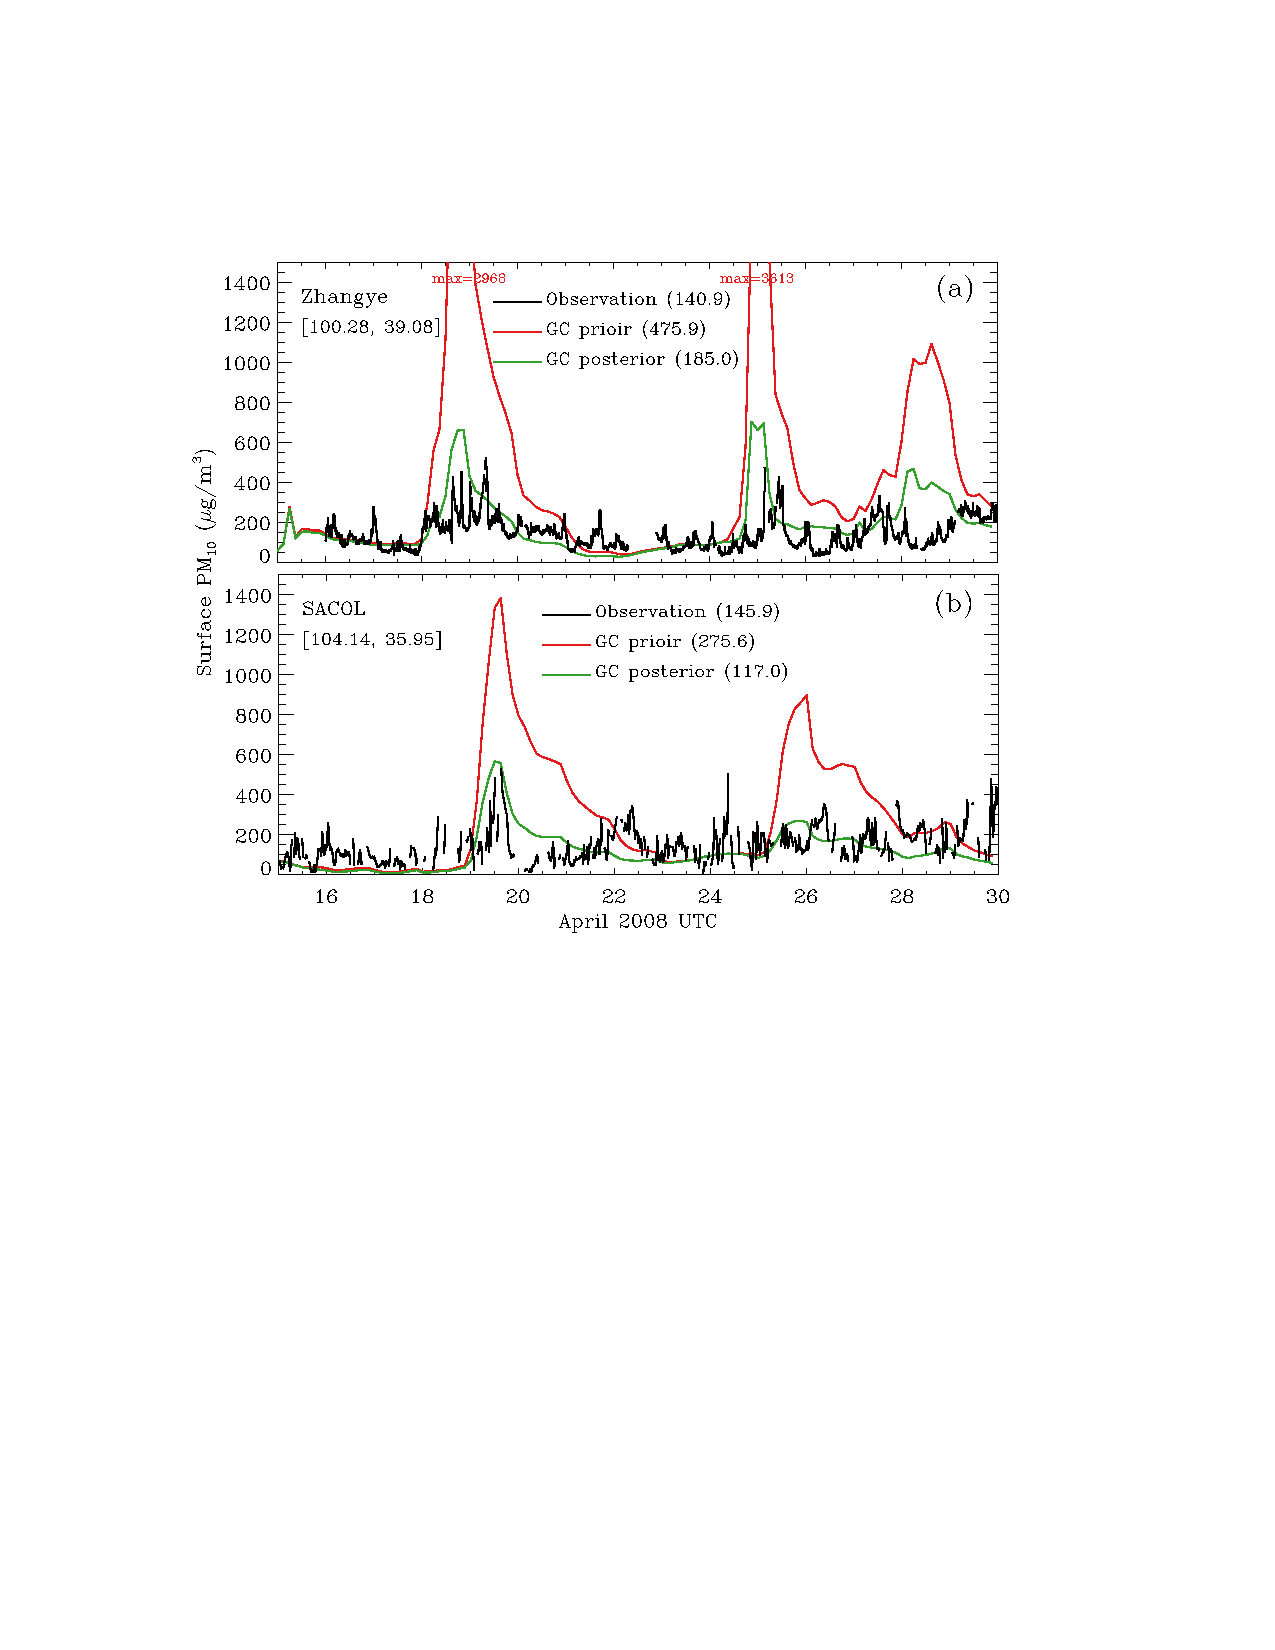
\includegraphics[width={0.95\textwidth}]{figures/a11.pdf}
  \caption{Time serial plot of the GEOS-Chem simulated surface PM\textsubscript{10} concentrations by prior (red) and posterior (red) aerosol emissions compared with the \textit{in situ} measured PM\textsubscript{10} (black) over Zhangye (a) and SACOL (b) stations for 15 – 30 April 2008; also shown are the average values over same the period. Discontinuity in time series is due to missing or quality filtered observations.}
  \label{fig:pm10}
 \end{figure}

 The mass concentration over or near the dust source regions
 where the anthropogenic emissions are small is most sensitive to the dust mass loading,
 and thus can be an indicator of the dust emissions in the first order.
 Figure \ref{fig:pm10} shows the prior and posterior GEOS-Chem surface
 PM\textsubscript{10} mass concentration compared with the ground-based measurements
 from the 2008 China-U.S. joint field experiment \citep{Ge10,Huang10} over two the AERONET sites
 in Figure \ref{fig:aeronet}a-b, i.e., Zhangye (100.28$^{\circ}$ E, 39.08$^{\circ}$ N)
 and SACOL (204.14$^{\circ}$ E, 35.95$^{\circ}$ N), which are located
 on the downwind boundaries of the Gobi deserts.
 Based on the availability of the measurements data, comparisons are for the period of 15--30 April 2008.
 The measured surface PM\textsubscript{10} shows a strong daily variation.
 A strong dust event during 18--20 April can be found over both stations with
 PM\textsubscript{10} exceeding 400 $\mu$g m$^{-3}$.
 Two additional dust events with PM\textsubscript{10} over 400 $\mu$g m$^{-3}$ occurred during
 24--26 and 29--30 April.
 The prior simulation generally captures the daily variation pattern
 but significantly overestimates the surface PM\textsubscript{10} for those dust events;
 prior simulated PM\textsubscript{10} reaches up to around 3000 $\mu$g m$^{-3}$ over Zhangye
 and 1000 $\mu$g m$^{-3}$ over SACOL for the dust events during 18$-$20 and 24$-$26 April 2008.
 The two-week averages show the prior simulation overestimates PM\textsubscript{10}
 a factor of 2 over Zhangye and a factor of 1 over SACOL in the magnitude.
 After optimization, the relative biases in the PM\textsubscript{10} simulation are reduced to about 25\%.
 Moreover, the comparison of the time series of the PM\textsubscript{10} also shows that
 the model value with top-down emissions has much better agreement
 with the measurements in terms of temporal variation.

 \subsection{Evaluation summary}

 A summary of evaluations of the prior and posterior model simulations
 is illustrated in Figure \ref{fig:taylor} using a Taylor diagram \citep{Taylor01}.
 Taylor diagram provides a statistical summary of the model performance
 in terms of correlation coefficients (R), centralized root-mean-square difference (RMSD),
 and ratio of standard deviations between model and observations (or normalized standard deviation, NSD).
 The latter two quantities reflect how well model captures
 the temporal or/and spatial variation of observations.
 In the Taylor diagram, cosine of polar angles represents R, and radius (dotted-contour) indicates NSD.
 Thus, the reference point (black circle) where R and NSD are unity represents observations,
 and the distance (dashed-contour) of certain point from which indicates the RMSD.
 Considering that the Taylor diagram itself is not able to show the statistical bias,
 we use different colors for each data points to indicate their respective relative biases.
 The data points labeled from 1 to 6 indicate comparisons between model and observations of
 (1) AERONET AOD at 0.55 $\mu$m,
 (2) MISR 0.55 $\mu$m AOD,
 (3) OMI retrievals of \ce{SO2} Column,
 (4) OMI retrievals of \ce{NO2} Column,
 (5) surface concentration of SNA over Qingdao, and
 (6) surface concentration of PM\textsubscript{10} over Zhangye and SACOL, respectively.
 Square and circles represent the evaluations for prior and posterior GEOS-Chem simulations, respectively.

 %% Validation Taylor diagram
 \begin{figure}[t]
  \centering
  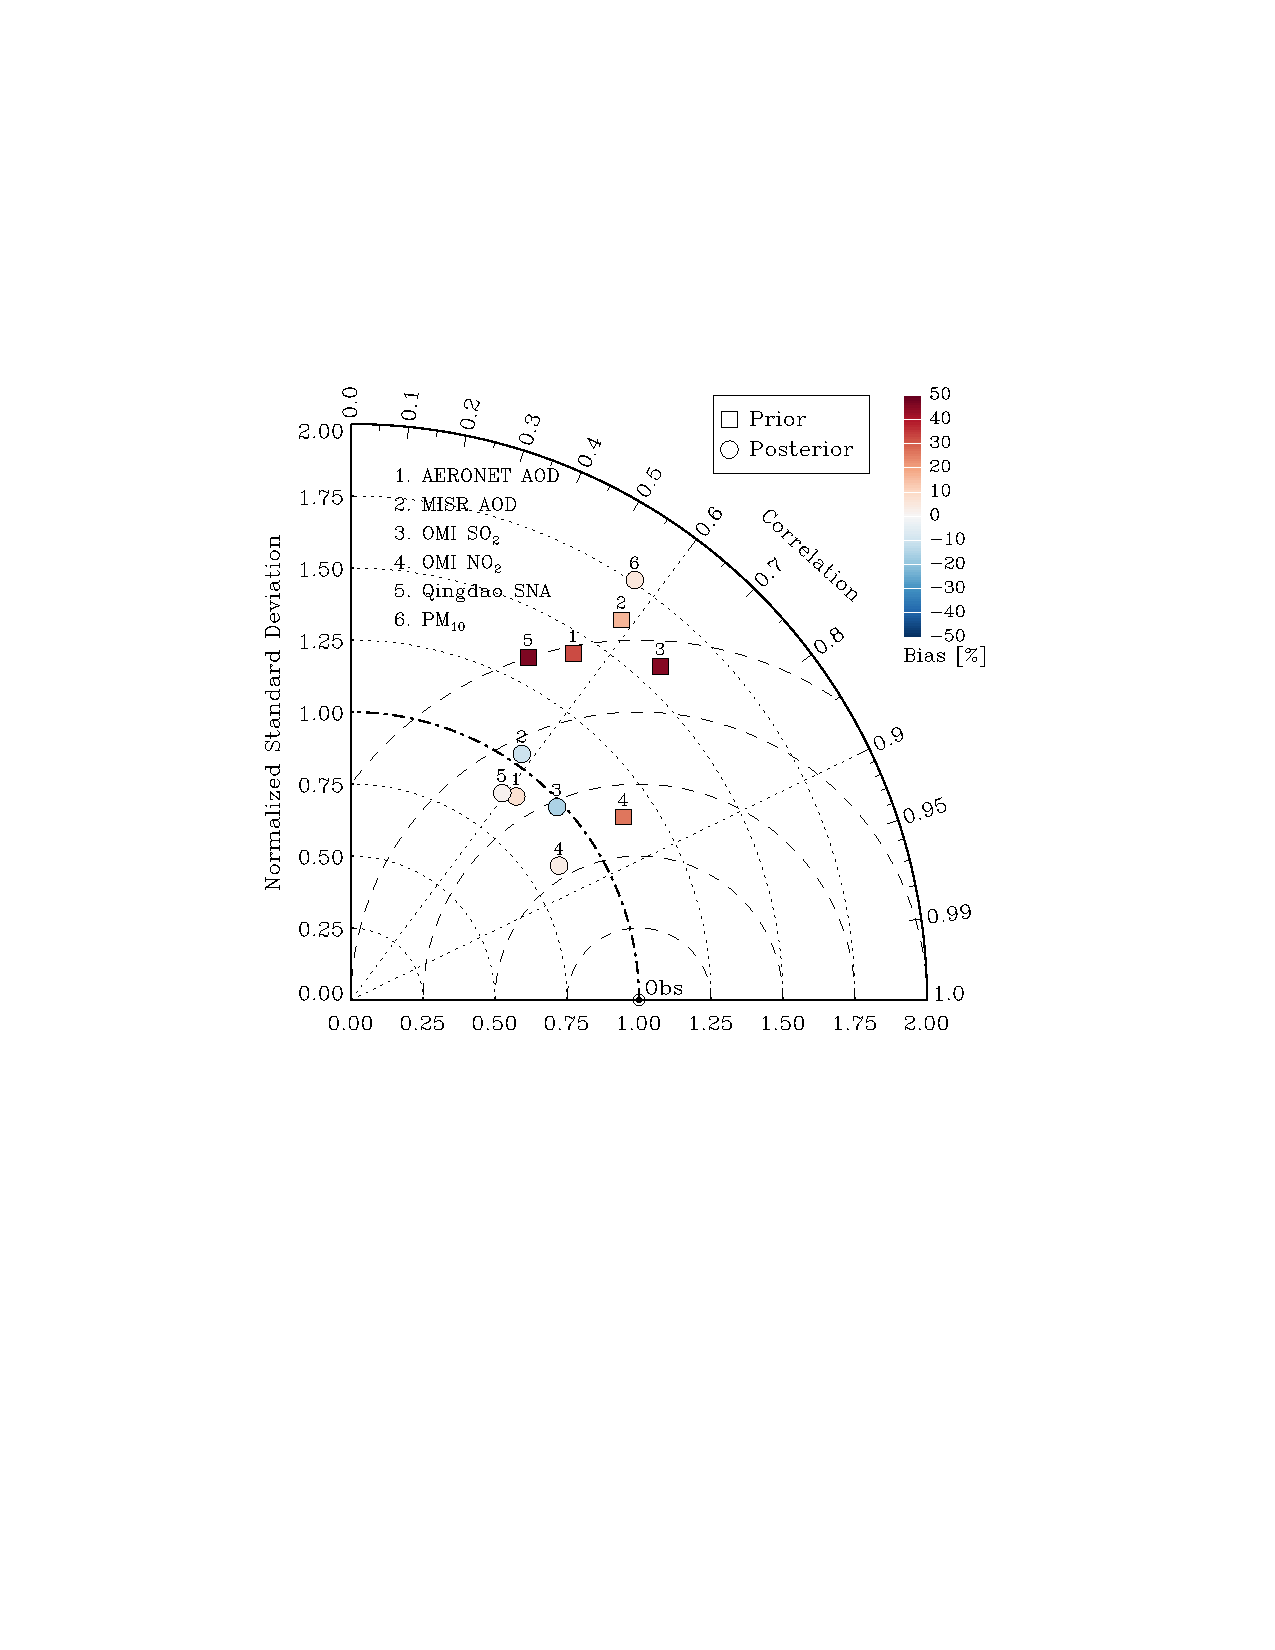
\includegraphics[width={0.66\textwidth}]{figures/a12.pdf}
  \caption{Taylor diagram for the model evaluations before (squares) and after (circles) optimization when comparing against (1) AERONET AOD at 0.55 $\mu$m, (2) MISR 0.55 $\mu$m AOD, (3) OMI column \ce{SO2}, (4) OMI column \ce{NO2}, (5) surface SNA concentrations at Qingdao site, and (6) surface PM\textsubscript{10} concentrations measured at Zhangye and SACOL sites. The color coded on each point indicates the relative bias. It should be noted that the ratio of standard deviations and correlation coefficient between prior GEOS-Chem simulated and measured surface PM\textsubscript{10} over Zhangye and SACOL are 6.5 and 0.45, which makes the point number 6 for the prior simulation far beyond the range of this Taylor diagram. }
  \label{fig:taylor}
 \end{figure}

 It should be noted that the NSD between prior GEOS-Chem simulated
 and measured surface PM\textsubscript{10} during the China-U.S. joint field campaign
 is about 6.5 (and R of 0.45) that are significantly beyond the range of this Taylor diagram.
 Consequently, the square point of number 6 is not shown in the diagram.
 It is clear from the Taylor diagram that the circular points (posterior simulation)
 are generally closer than the square points (prior simulation) to the reference point
 and to the unity curve of NSD, and have remarkably decreased bias.
 Evaluations with all those independent observations indicate a notable
 improvement in the model simulation, reflecting a better estimate of aerosol emissions.

\section{Implications of Results} \label{sec:invimplication}

  Interpretation of our inversion results can be from two different perspectives. 
First, if assuming that bottom-up anthropogenic emissions are the best estimates for their base years (mostly 2006), 
the reduction in the top-down emissions over China for April 2008 may indicate a decrease of emissions for April from 2006 to 2008. 
This conjecture is supported by the finding of significant decrease of AOD from 2006 to 2008 over the eastern China, 
shown both in the MODIS and MISR Level 3 gridded products (Figure \ref{fig:aodchange}),
if we assume that the impact on AOD of meteorological differences between the two years is smaller than the differences in emissions.
Furthermore, a slight increase of AOD over the Southeastern China (Figure \ref{fig:aodchange}) 
is also found to be consistent to the increase in the top-down emission estimates (Figure \ref{fig:ems1}). 
In contrast to the first interpretation, the second one is that the difference of actual emissions between 2008 and their base year (2006)
are smaller than the magnitude of adjustments in the optimization, 
and hence our results imply that the priori bottom-up emissions might be artificially overestimated. 
We further elucidate those two points below with a literature survey (data are summarized in Table \ref{tab:emssurvey}).

 %% Satellite AOD changes
 \begin{figure}[t]
  \centering
  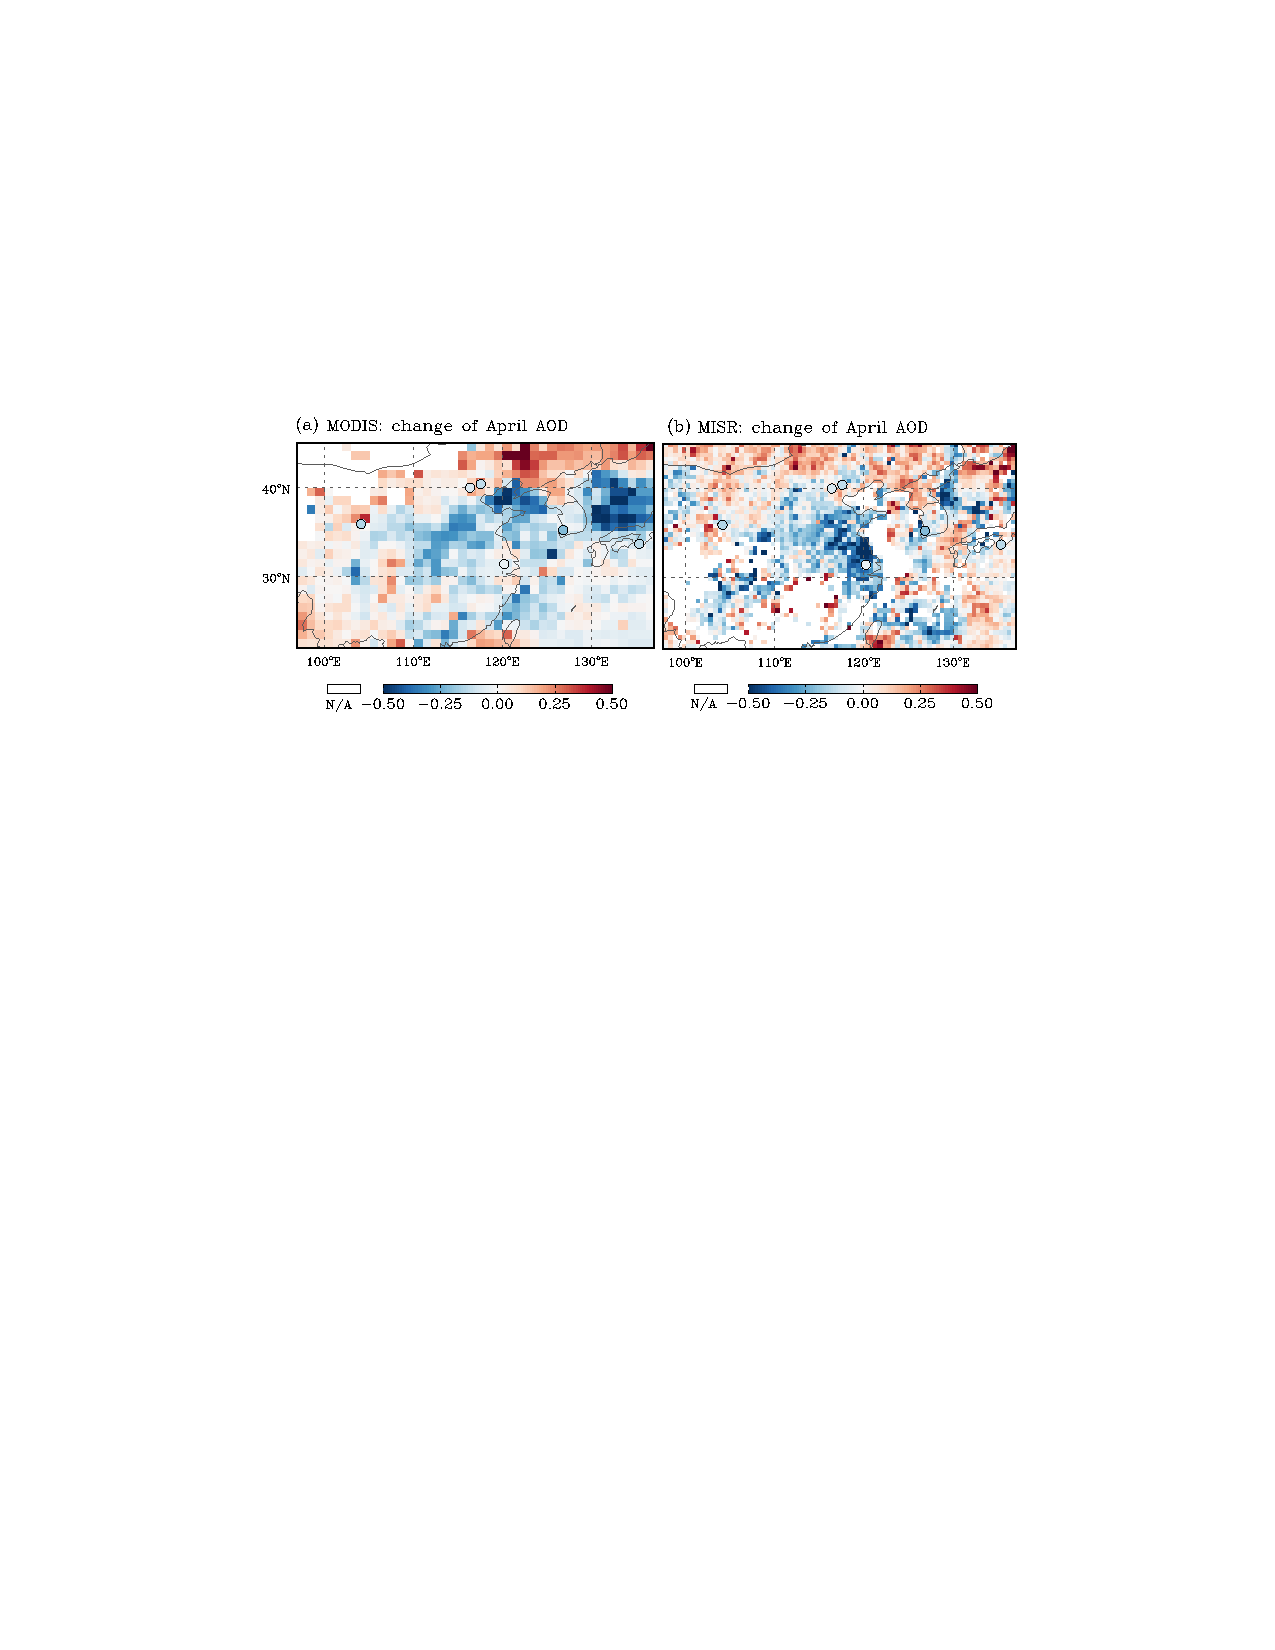
\includegraphics[width={0.90\textwidth}]{figures/a13.pdf}
  \caption{Change of April monthly 0.55 $\mu$m AOD from 2006 to 2008
from MODIS (a) and MISR (b) Level 3 daily products. \citep[Figure
adopted from][]{Xu13}}
  \label{fig:aodchange}
 \end{figure}

 \subsection{SO\textsubscript{2}}

  The INTEX-B inventory by \citet{Zhang09b} reported an annual production of 
31.02 Tg from anthropogenic sources over China. 
A decrease trend of China SO2 emissions from 2006 to 2008 has been found based
on bottom-up estimates by \citet{Lu10} from 33.2 to 31.3 ( $\sim$5.8\% decrease) Tg yr$^{-1}$
and by China \citet{MEP09} (hereafter referred to MEP-2008) from 25.9 to 
23.2 Tg yr$^{-1}$ ($\sim$10.4\% decrease).
With OMI \ce{SO2} retrievals, \citet{Lu10} found the dramatic reduction of 
\ce{SO2} emissions over the northern China for the same period. 
Similar to this study, \citet{Lu10} also presented that the reductions is more
significant over the Eastern China. They attribute some reduction to the 
widespread installation of flue-gas desulfurization devices in power plants,
which is enforced by the China government since 2006. 
Evidences for the reduction trend of \ce{SO2} emission also include the reduction 
of \ce{SO2} column from 2006 observed by both SCIAMACHY and OMI satellite sensors \citep{Lu11}.
With the same SCIAMACHY and OMI \ce{SO2} retrievals, \citet{Lee11} obtained 
top-down estimates of China SO2 emissions, which are lower by 50\% for 
SCIAMACHY and 30\% for OMI than the INTEX-B inventory. 
Thus, the reduction of 33.5\% in the top-down China \ce{SO2} emissions of this 
work can be interpreted by the joint contribution of a decrease trend and a 
possible overestimation in INTEX-B bottom-up inventory.

 \subsection{NH\textsubscript{3} } 

  The \ce{NH3} emissions over China have not changed much since 2000, as 
confirmed by the REAS inventory \citep{Ohara07}. Our study shows an overall 
decrease of 34.5\% in the optimized from the TRACE-P 2000 inventory \citep{Streets03},
which may indicate an overestimation in the TRACE-P inventory. 
As shown in Table \ref{tab:emssurvey}, the total amount of the constrained 
\ce{NH3} emission (0.72 Tg Mon$^{-1}$) for April 2008 is quite close to a 
recent bottom-up estimates (0.71 Tg Mon$^{-1}$) by \citet{Huang12}. 
\citet{Huang12} also pointed out that the TRACE-P 2000 inventory significantly
overestimates the \ce{NH3} emission by applying an overestimated emission 
factor across the whole country. 

\begin{table}[t]
  \centering
  \small
  \caption{Comparisons for annually (Tg yr$^{-1}$) and/or for April only (Tg Mon$^{-1}$) estimates of Chinese aerosol emissions during 2006 and 2008.}
  \label{tab:emssurvey}
  \begin{tabular}{m{3em} m{14em} C{3em} C{3em} C{0.5em} C{3em} C{3em} }
    \toprule
    \multicolumn{2}{l}{} & \multicolumn{2}{c}{2006} & \multicolumn{1}{c}{} & \multicolumn{2}{c}{2006}      \\
    \cline{3-4} \cline{6-7}
    Tracer &  Emission inventories & Annual & April & & Annual\textsuperscript{a} & April \\
    \midrule
             & INTEX-B \citep{Zhang09b} & 31.02 & 2.37 & & -     & - \\
    \ce{SO2} & China MEP-2008           & 25.89 & -    & & 23.21 & - \\ 
             & \citet{Lu10}             & 33.2  & -    & & 31.3  & - \\
             & This work                & -     & 2.60 & & 22.69 & 1.73 \\
    \midrule
             & TRACE-P \citep{Streets03} & 13.6 & 1.10 & & -     & - \\
    \ce{NH3} & \citet{Huang12}           & 9.8  & 0.71 & & -     & - \\
             & This work                 & -    & 1.10 & & 8.91  & 0.72 \\
    \midrule
             & INTEX-B \citep{Zhang09b} & 20.83 & 1.63 & & -     & - \\
    \ce{NOx} & \citet{Lin10}            & -     & -    & & 22.34 & - \\
             & This work                & -     & 1.69 & & 17.60 & 1.38 \\
    \midrule
             & INTEX-B \citep{Zhang09b} & 1.81  & 0.12 & & -     & - \\
             & \citet{Qin12}            & 1.55  & -    & & 1.61  & - \\
    BC       & \citet{Lu11}             & 1.63  & -    & & 1.68  & - \\
             & \citet{Zhao13}           & 1.60  & -    & & 1.60  & - \\
             & This work                & -     & 0.11 & & 1.51  & 0.10 \\
    \midrule
             & INTEX-B \citep{Zhang09b} & 3.22  & 0.19 & & -     & - \\
    OC       & \citet{Lu11}             & 3.42  & -    & & 3.37  & - \\
             & \citet{Zhao13}           & 2.90  & -    & & 2.80  & - \\
             & This work                & -     & 0.21 & & 2.92  & 0.18 \\
    \bottomrule
    \multicolumn{6}{m{29em}}{\textsuperscript{a}Our annual top-down estimates (Tg yr$^{-1}$) are based on the monthly variation of the INTEXT-B inventory.} 
  \end{tabular}
\end{table}


 \subsection{NOx} 

  \citet{lin10} constrained Chinese anthropogenic emissions of \ce{NOx} in 
July 2008 with tropospheric \ce{NO2} retrievals from GOME-2 and OMI instruments.
They found the top-down emissions are (10$-$15\%) lower than the 
\textit{a priori} near Beijing (in agreement with results from \citet{Mijling09}),
in the northeastern provinces and along the east coast; yet they exceed 
the \textit{a priori} over many inland regions. Overall, they presented a best
top-down estimate of annual \ce{NOx} production is 6.8 Tg N, or 22.34 Tg NO2, 
which is slightly higher than the \textit{a priori}. 
While the change in \ce{NOx} emission over China remains controversy, 
the 18.8\% difference of posterior NOx emissions from the bottom-up still 
lies in the 31\% uncertainty of the inventory \citep{Zhang09b}. We argue 
bottom-up \ce{NOx} estimate from INTEX-B inventory could have a possible 
overestimation.   

 \subsection{BC and OC}  

  Major emitting sectors of BC and OC are coal and biofuel combustion by 
industry, residential, and transportation activities. 
The trend of BC and OC emissions in China during recent years are controlled 
by the balance between decrease in emission factor which is pertain to 
improved technology and increase in coal and fuel consumptions. 
According to MEP-2008 \citep{MEP09}, the annual smoke emission in China 
decreased by about 17.2\% from 2006 to 2008. 
While BC and OC emissions estimated by \citet{Lu11} and \citet{Zhao13} remain 
almost same between 2006 and 2008, \citet{Qin12} reported a 3.8\% increase. 
The top-down BC emission is 0.10 Tg mon$^{-1}$ (or 1.509 Tg yr$^{-1}$ based on 
the monthly variation in INTEX-B inventory), which is smaller than that in 
INTEX-B, but close to estimates of 1.61 Tg yr$^{-1}$ by \citet{Qin12} and 
1.68 Tg yr$^{-1}$ by \citet{Lu11}. In terms of China OC emission estimates 
for 2008, \citet{Lu11} suggested a slightly larger value (3.37 Tg yr$^{-1}$) 
while \citet{Zhao13} indicated a smaller value (2.8 Tg yr$^{-1}$) than 
INTEX-B (3.22 Tg yr$^{-1}$). Our OC emission estimate (0.18 Tg mon$^{-1}$ or 
2.92 Tg yr$^{-1}$) is within their reported range. It is noted that the 
uncertainty for OC emissions is reported to be very large: 258\% in INTEX-B 
\citep{Zhang09b}, $-$43\% to 80\% by \citet{Lu11}, and $-$42\% to 114\% 
by \citet{Zhao13}.

 \subsection{Mineral dust} 

  The $\sim$50\% reduction in the posterior dust emission estimates suggests 
the use of DEAD mobilization scheme with GOCART source function possibly tends
to produce a systematic positive bias over the Taklimakan and Gobi deserts 
regions over the northwestern China, even it works reasonably for the United 
States \citep{Fairlie07}. Similar results have been also found in top-down 
dust emission estimates by MODIS aerosol retrievals \citep{Wang12}, 
and constrained dust emissions by surface PM measurements \citep{Ku11}. 
Such overestimation by the dust mobilization scheme is also reflected through
comparison GEOS-Chem AOD (as in Figure \ref{fig:aeronet}) and surface 
PM\textsubscript{10} conentration (as in Figure \ref{fig:pm10}) with
\textit{in situ} measurements near the dust source regions. 


\section{Summary} \label{sec:invsummary}

 This study presents a two-stage inversion scheme to explore the capacity of 
using satellite radiance for inversion of species-specific aerosol emissions.
Firstly, we prepare the observational constraints of AOD using an advanced 
aerosol retrieval algorithm, which integrates the GEOS-Chem aerosol optical 
properties to the MODIS observed radiance \citep{Wang10}.
Secondly, the adjoint of the GEOS-Chem chemical transport model is applied to 
statistically optimize aerosol emission estimates using these AOD retrievals.
Thus, the MODIS radiances are essentially used to optimize the estimates of 
the emitted aerosol tracers and precursors.

We illustrate our concept first with an idealized numerical experiment,
 and subsequently demonstrate the feasibility and practicability of the 
proposed scheme by applying it to optimize aerosol emission inventories over
China during April 2008. Emissions of \ce{SO2}, \ce{NH3}, \ce{NOx}, BC and OC 
from anthropogenic sources, which significantly influence the aerosol 
simulation, are selected to be constrained at a spatial resolution of 
2$^{\circ}$ by 2.5$^{\circ}$ and a monthly temporal resolution.
Mineral dust production from combined natural and disturbed sources are 
optimized at the same spatial resolution but with a daily temporal resolution.
Independent observations from both satellite remote sensing and ground-based 
observations are used to assess the inversion results through their 
comparisons with relevant GEOS-Chem simulations using prior and posterior 
emission estimates. 

The inversion yields posterior best estimates of 1.73 Tg for \ce{SO2}, 0.72 Tg
for \ce{NH3}, 1.38 Tg for NOx, 0.10 Tg for BC, and 0.18 for OC from 
anthropogenic sources, and 8.3 Tg for combined natural and disturbed mineral 
dust. These show notable decreases from their counterparts in the bottom-up 
inventories in amount (or percentage decrease): 0.87 Tg (33.5\%) for \ce{SO2},
0.38 Tg (34.5\%) for \ce{NH3}, 0.32 Tg (18.8\%) for \ce{NOx}, 0.01 Tg (9.1\%) 
for BC, and 0.03 Tg (15.0\%) for OC. The total amount of the mineral dust 
emission is reduced by 56.4\% from 19.02 Tg simulated by the DEAD mobilization
module. The distribution of emission scaling factors exhibits strong spatial
variation for those anthropogenic-emitted tracers and considerable temporal
variation for mineral dust. The use of top-down constrained emissions 
remarkably reduces the discrepancy between GEOS-Chem simulation and 
observational AOD constraints, in both spatial and temporal variation
features.

 Resulting posterior estimates of emissions are evaluated with independent 
AOD observations from surface sites (AERONET) and satellite (MISR), \ce{SO2} 
and \ce{NO2} column retrievals from satellite (OMI), and surface SNA and 
PM\textsubscript{10} concentrations from ground-based measurements. While the
prior simulation over China generally shows overestimation, the use of
posterior emissions significantly enhances the consistency between simulations
and those independent observations. The statistical analysis of those 
comprehensive comparisons summarized in the Taylor diagram shows an
overall reduced bias and root-mean-squre difference along with increased
correlation coefficient, further confirming the improvements in the
posterior simulation and the effectiveness of the presented top-down
scheme.

 We attribute the differences between prior and posterior aerosol
emissions to the change of emitted amount from the base year of those
bottom-up inventories to the study period and/or the
under/over-estimations in those inventories. Through comparisons with
emissions over China reported by recent studies, we find that our
inversion results are consistent with following finding:
 \begin{itemize}
 \item Anthropogenic \ce{SO2} emissions over China has been decreased by
5$-$10\% from 2006 to 2008;
 \item Anthropogenic BC/OC emissions may be slightly reduced;
 \item Anthropogenic emissions of \ce{SO2} and \ce{NOx} reported in the
INTEX-B and \ce{NH3} from TRACE-P inventories could have been
artificially overestimated;
 \item The DEAD mobilization scheme combined with GOCART dust source
function, even works well over the United State \citep{Fairlie07}, seems
to simulate mineral dust surface fluxes with a systematic positive bias.
 \end{itemize}
  
 As a first attempt to invert species-specific emissions with satellite
radiance, this study has a number of limitations. Those limitations may
impact the uncertainty in posterior emissions, which is supposed to be
smaller than uncertainty characterizing either a priori or observational
constraints \citep{Rodgers00}. While quantification of these is beyond
the demonstrative purposes of this paper, we present a qualitative
discussion as follows. First, in the stage of aerosol retrieval, we
presume aerosol composition is unbiased, and contains errors only in the
total amount. As the model inevitably has bias associating aerosol
types, improvement of this assumption over regional to global scale can
be obtained from innovative satellite measurements. Indeed, the radiance 
observations have potential information on the aerosol composition.
For example, the spectral behavior of the radiance is used to
discriminate smoke from mineral dust particles\citep{King99, Kaufman02}.
Radiances measured from multi-viewing-angle are sensitive to aerosol 
particle size and nonsphericity \citep{Martonchik09}.
Temporal variation and geographical location can also yield information 
about aerosol composition. For example, increase of AOD in semi-arid
region may reflect the increase of dust, while change of AOD in the
Eastern Asia may reflect the increase of industrial emission.
Hence, as showed in this study, a combined use of the model-based
knowledge of the dominant aerosol sources and the source-receptor
relationship together with the satellite-based temporal variation of AOD
at different locations can be a strong constraint for species-specific
source estimates. Second, this study also assumes the sole cause of the
radiance difference (or the AOD difference) is due to the uncertainty in
aerosol emissions. However, other processes can contribute to the
difference, e.g. aerosol transport, wet/dry deposition, diurnal
variation, prescribed aerosol physical and optical properties, and
errors in the meteorological fields and radiative transfer calculation,
etc. The third assumption is related to the error covariance matrices
that are specified as diagonal with errors based upon literature (but
that themselves may have uncertainty). To properly address these issues
in future, a logical next step would be to assimilate multiple-spectral
and/or multi-angle satellite radiance to the CTM. Furthermore, errors in
the processes including emission, transport, and deposition and
radiative transfer, should be reasonably characterized and included in
the optimization. 

The top-down inversion scheme using GEOS-Chem adjoint inverse modeling
is a powerful tool to include observational constraints from different
platforms for timely updating aerosol emissions. There is also a need of
using combined tracer gas and aerosol measurements to simultaneously
constrain the aerosol emissions and gas precursors.
Encouraging results presented in this study reveal the potential of
using aerosol observations from MODIS and MISR, \ce{SO2} and \ce{NO2}
from OMI and other sensor, such as SCIAMACHY, in the inversion.
Inclusion of those observations will undoubtedly add more information to
the optimization of emission.

